%-------------------------------------------------------------------------------
% This file provides a skeleton ATLAS note.
% \pdfinclusioncopyfonts=1
% This command may be needed in order to get \ell in PDF plots to appear. Found in
% https://tex.stackexchange.com/questions/322010/pdflatex-glyph-undefined-symbols-disappear-from-included-pdf
%-------------------------------------------------------------------------------
% Specify where ATLAS LaTeX style files can be found.
\newcommand*{\ATLASLATEXPATH}{latex/}
% Use this variant if the files are in a central location, e.g. $HOME/texmf.
% \newcommand*{\ATLASLATEXPATH}{}
%-------------------------------------------------------------------------------
\documentclass[NOTE, atlasdraft=true, texlive=2016, UKenglish]{\ATLASLATEXPATH atlasdoc}
% The language of the document must be set: usually UKenglish or USenglish.
% british and american also work!
% Commonly used options:
%  atlasdraft=true|false This document is an ATLAS draft.
%  texlive=YYYY          Specify TeX Live version (2016 is default).
%  coverpage             Create ATLAS draft cover page for collaboration circulation.
%                        See atlas-draft-cover.tex for a list of variables that should be defined.
%  cernpreprint          Create front page for a CERN preprint.
%                        See atlas-preprint-cover.tex for a list of variables that should be defined.
%  NOTE                  The document is an ATLAS note (draft).
%  PAPER                 The document is an ATLAS paper (draft).
%  CONF                  The document is a CONF note (draft).
%  PUB                   The document is a PUB note (draft).
%  BOOK                  The document is of book form, like an LOI or TDR (draft)
%  txfonts=true|false    Use txfonts rather than the default newtx
%  paper=a4|letter       Set paper size to A4 (default) or letter.

%-------------------------------------------------------------------------------
% Extra packages:
\usepackage{\ATLASLATEXPATH atlaspackage}
% Commonly used options:
%  biblatex=true|false   Use biblatex (default) or bibtex for the bibliography.
%  backend=bibtex        Use the bibtex backend rather than biber.
%  subfigure|subfig|subcaption  to use one of these packages for figures in figures.
%  minimal               Minimal set of packages.
%  default               Standard set of packages.
%  full                  Full set of packages.
%-------------------------------------------------------------------------------
% Style file with biblatex options for ATLAS documents.
\usepackage{\ATLASLATEXPATH atlasbiblatex}
% Commonly used options:
%  backref=true|false    Turn on or off back references in the bibliography.

% Package for creating list of authors and contributors to the analysis.
\usepackage{\ATLASLATEXPATH atlascontribute}

% Useful macros
\usepackage{\ATLASLATEXPATH atlasphysics}
% See doc/atlas_physics.pdf for a list of the defined symbols.
% Default options are:
%   true:  journal, misc, particle, unit, xref
%   false: BSM, heppparticle, hepprocess, hion, jetetmiss, math, process,
%          other, snippets, texmf
% See the package for details on the options.

% Files with references for use with biblatex.
% Note that biber gives an error if it finds empty bib files.
%\addbibresource{FCNCtqaINT.bib}
%\addbibresource{bib/ATLAS.bib}
%\addbibresource{bib/CMS.bib}
%\addbibresource{bib/ConfNotes.bib}
%\addbibresource{bib/PubNotes.bib}

% Paths for figures - do not forget the / at the end of the directory name.
\graphicspath{{logos/}{figures/}}

% Add you own definitions here (file FCNCtqaINT-defs.sty).
\usepackage{FCNCtqaINT-defs}

%-------------------------------------------------------------------------------
% Generic document information
%-------------------------------------------------------------------------------
\usepackage{amsmath}
\usepackage{slashed}
\usepackage{hhline}
\usepackage{tabularx}
% Title, abstract and document 
%-------------------------------------------------------------------------------
% This file contains the title, author and abstract.
% It also contains all relevant document numbers used for an ATLAS note.
%-------------------------------------------------------------------------------

% Title
\AtlasTitle{AtlasTitle: Bare bones ATLAS document}

% Draft version:
% Should be 1.0 for the first circulation, and 2.0 for the second circulation.
% If given, adds draft version on front page, a 'DRAFT' box on top of each other page, 
% and line numbers.
% Comment or remove in final version.
\AtlasVersion{0.1}

% Abstract - % directly after { is important for correct indentation
\AtlasAbstract{%
  This is a bare bones ATLAS document. Put the abstract for the document here.
}

% Author - this does not work with revtex (add it after \begin{document})
%\author{Jason Barkeloo}

% Authors and list of contributors to the analysis
% \AtlasAuthorContributor also adds the name to the author list
% Include package latex/atlascontribute to use this
% Use authblk package if there are multiple authors, which is included by latex/atlascontribute
 \usepackage{authblk}
% Use the following 3 lines to have all institutes on one line
 \makeatletter
 \renewcommand\AB@affilsepx{, \protect\Affilfont}
 \makeatother
 \renewcommand\Authands{, } % avoid ``. and'' for last author
 \renewcommand\Affilfont{\itshape\small} % affiliation formatting
 \AtlasAuthorContributor{Jason Barkeloo}{a}{All Aspects}
% \AtlasAuthorContributor{Second AtlasAuthorContributor}{b}{Author's contribution.}
% \AtlasAuthorContributor{Third AtlasAuthorContributor}{a}{Author's contribution.}
% \AtlasContributor{Fourth AtlasContributor}{Contribution to the analysis.}
% \author[a]{Jason Barkeloo}
%% \author[a]{Second Author}
% \author[b]{Third Author}
 \affil[a]{University of Oregon}
%% \affil[b]{Another Institution}

% If a special author list should be indicated via a link use the following code:
% Include the two lines below if you do not use atlasstyle:
% \usepackage[marginal,hang]{footmisc}
% \setlength{\footnotemargin}{0.5em}
% Use the following lines in all cases:
% \usepackage{authblk}
% \author{The ATLAS Collaboration%
% \thanks{The full author list can be found at:\newline
%   \url{https://atlas.web.cern.ch/Atlas/PUBNOTES/ATL-PHYS-PUB-2017-007/authorlist.pdf}}
% }

% ATLAS reference code, to help ATLAS members to locate the paper
\AtlasRefCode{GROUP-2017-XX}

% ATLAS note number. Can be an COM, INT, PUB or CONF note
% \AtlasNote{ATLAS-CONF-2017-XXX}
% \AtlasNote{ATL-PHYS-PUB-2017-XXX}
% \AtlasNote{ATL-COM-PHYS-2017-XXX}

% Author and title for the PDF file
\hypersetup{pdftitle={ATLAS document},pdfauthor={The ATLAS Collaboration}}

%-------------------------------------------------------------------------------
% Content
%-------------------------------------------------------------------------------
\begin{document}

\maketitle

\tableofcontents

% List of contributors - print here or after the Bibliography.
%\PrintAtlasContribute{0.30}
%\clearpage


%-------------------------------------------------------------------------------
\newpage
\section{Change Log}
\label{sec:change}
%-------------------------------------------------------------------------------
\textbf{Version 0.1}
\begin{itemize}
\item First Draft
\end{itemize}

%-------------------------------------------------------------------------------
%\newpage
%\section{Introduction}
%\label{sec:intro}

\chapter{Introduction}
\label{ch:Introduction}
%Deep thoughts go here.
Over the last 50 years, the Standard Model of particle physics has proven itself time and time again, successfully describing phenomena covering several orders of magnitude in energy as well as describing new particles, such as the Higgs boson, which was finally discovered in 2012.  However, this spectacular resilience is also a source of great frustration.  The Standard Model is known to be incomplete, lacking answers for neutrino masses, the mass of the Higgs boson, dark matter...yet every precision search has yet to poke any new holes in it.  With the Large Hadron Collider (LHC) reaching a new center of mass energy in 2015, the hope is to discover new particles which only become accessible at very high energies.

As a hadron collider, the LHC produces collisions which are dominated by strongly interacting particles which are detected in the form of jets.  Given this very high cross-section, the dijet search is positioned to take advantage of the extraordinary statistics to look for evidence of strongly interacting new resonances across a very large mass range, and hopefully pointing the way for precision searches to explore any excesses that are seen.

This thesis presents the resonance portion of the dijet analysis performed on the combined 2015 and 2016 datasets taken by the ATLAS experiment.\cite{Dijet2017}  The analysis looks at the dijet invariant mass spectrum for evidence of localized excesses which could point to new resonances or other forms of physics beyond the Standard Model.  The analysis uses a model-agnostic methodology to be sensitive to as many possible Beyond the Standard Model (BSM) models as possible, and its results are presented both in terms of limits on selected benchmark models as well as for generic Gaussians which can be used to interpret limits for other theoretical models.

This research paper result was by no means an individual effort, but was built on the efforts of dozens of other researchers, both past and present.  The author's individual contributions included maintenance of the core analysis code, preparation, processing, and dissemination of real and simulated data samples, Wilks' statistical testing, year-to-year dataset validation, and serving as analysis contact and paper editor.  Chapters VII and VIII contain work previously published in Physical Review D, Volume 96, on September 28th, 2017.\cite{Dijet2017}  Chapter IX contains work which has been made public, some of which is awaiting publication.\cite{DijetISR_Resolved}\cite{DijetTLA}\cite{DijetISR}  These works are co-authored with the ATLAS Collaboration, comprising approximately 2900 authors, the full list of which are available in the full publications.

Chapter~\ref{ch:Theory} introduces the Standard Model as well as the benchmark models used in the analysis.  Chapters~\ref{ch:Detector} and~\ref{ch:Calorimetry} discuss the Large Hadron Collider and ATLAS Experiment, with a special focus on the calorimetry systems used to measure jets.  Chapter~\ref{ch:Jets} covers the strong force and how it gives rise to the jets measured in this analysis, while Chapter~\ref{ch:Calibration} discusses how jets are reconstructed and calibrated into final physics objects.  Chapter~\ref{ch:SearchStrategy} covers the search strategy used in this analysis and the sources of uncertainty in the result.  Finally, Chapter~\ref{ch:Results} discusses the finding and limits set on models of new physics while Chapter~\ref{ch:Conclusion} puts these limits in context of other complementary searches as well as the future outlook.


%-------------------------------------------------------------------------------
\newpage
\section{Object Reconstruction}
\label{sec':ObjReco}
After the events are simulated, or collected in case of real data, the collections of energy deposits within the detector systems must be transformed into meaningful physics objects through reconstruction.  Reconstruction is typically done in two major parts using the specialized detectors covered in Chapter \ref{ch:LHCDetector}.  The Inner Detector and Muon System turn patterns of hits within the tracking detectors into tracks that have direction and momentum information.  The calorimeter system transforms the energy deposits within the calorimeters into calibrated energy deposits with a particular position.  These tracks and calorimeter deposits are used to create physics objects (electrons, muons, etc.) by using particle identification techniques to reconstruct the underlying physics event.  For the analysis presented in this dissertation, the final state signal particles that need to be reconstructed are one lepton (an electron or a muon), one photon, two quarks (one light flavor and one b quark), and one neutrino (missing transverse energy as it is the only particle that does not interact with the detector).  Each of these particles has a particular signature in the subdetectors of the ATLAS detector, shown in Figure \ref{fig:ATLASInteractions}.

\begin{figure}[h]
	\centering
	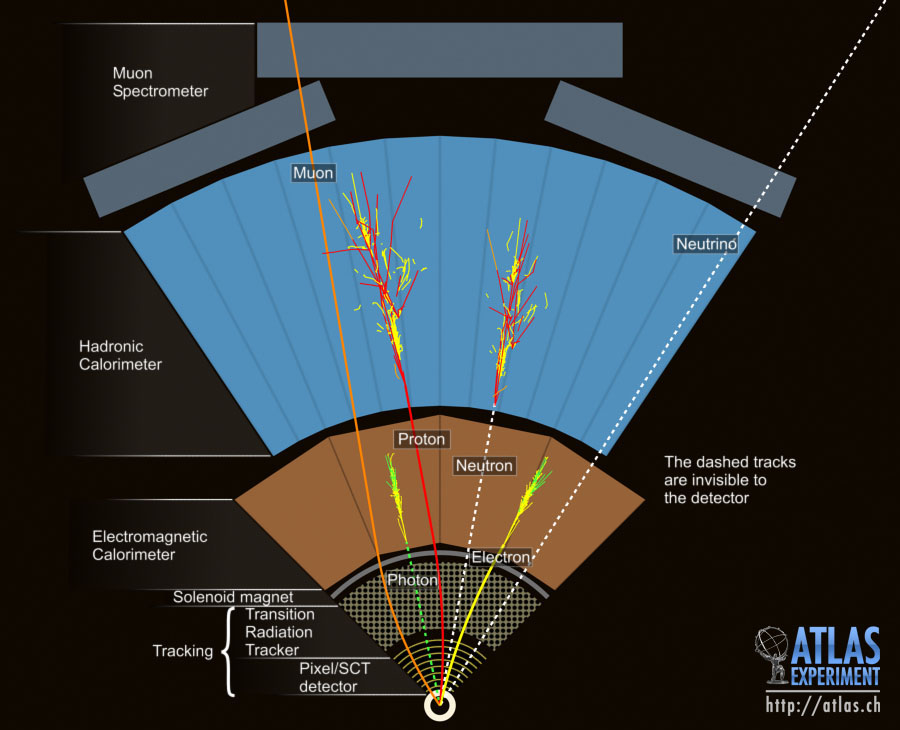
\includegraphics[width=\columnwidth]{../ThesisImages/Simulation/ParticleInteractions.jpg}
	\caption[Cross section of a simulated ATLAS detector showing how various particles interact with ATLAS subsystems.]{Cross section of a simulated ATLAS detector showing how various particles interact with ATLAS subsystems.  Solid lines indicate interactions while dashed lines indicate that no interactions typically occur in that section of the detector. \cite{ParticleInteractions} 
	}
	\label{fig:ATLASInteractions}
\end{figure}


\subsection{Electrons}
Electrons interacting with within the ATLAS detector leave a track in the Inner Detector as well as a cluster of energy in the electromagnetic calorimeter.  The track and cluster are required to be matched together to be identified as an electron candidate\cite{ElectronID}.  As electrons move through the detector they create electromagnetic showers through bremsstrahlung which can produce electron-positron pairs.  The process continues as the particles continue to give energy to the detector.  This collection of electrons, positrons, and photons creates a signature energy cluster in the calorimeter.  

Electron identification algorithms are applied to the electron candidates to separate prompt and isolated electron candidates from electrons that come from backgrounds such as converted photons and misidentified jets.  The electron idenification algorithms use a sliding window ( $3\times5$ in $\eta \times \phi$) in the high granularity section of the LAr electromagnetic calorimeter to search for electron cluster ``seeds'' greater than 2.5 GeV.  Clusters are created around these seeds to form the electromagnetic shower and remove possible duplicate electron signals by containing them within the cluster.  Further pattern recognition for the track fitting allows even larger amounts of energy into the shower to account for bremsstrahlung in the shower shape.  Tracks and clusters are then matched to give electron candidates.  

Electrons coming from background jets or photon conversion are called non-prompt as they do not originate from a signal object/the primary vertex.  In order to reject these electrons, other discriminating variables are used in addition to the track-cluster matching.  These variables inclue the amount of energy leakage into the hadronic calorimeter, thee shower development throughout the electromagnetic calorimeter, and the amount of radiation measured in the TRT.  Three electron identification working points are used: Loose, Medium, and Tight.  Each of these operating points have their own level of background rejection and signal efficiency.  Working points with higher background rejection are a subset of those with lower background rejection.

Isolation variables are another useful tool in the identification of signal electrons from converted photons produced in hadron decays and light hadron misidentification.  These variables are defined by a cone size around the electron candidate and are the sum of the transverse variable (momentum or energy) of all of the tracks within the cone, $p_{T}^{\text{cone0.2}}$ with a cone of $\Delta R =0.2$ (or 10 GeV/$E_T$, for high energy electrons) and $E_{T, Topo}^{\text{varcone0.4}}$ with a cone defined in a similar manner.  

Because the LAr calorimeter is a sampling calorimeter, the energy deposits must be calibrated and scaled such that the true electron energy is read out and not just the small amount of energy deposited into the active layers as discussed in Section \ref{sec:EMHCal}.  The energy scale is calibrated to be uniform throughout the detector.  Any residual differences between data and simulation are corrected.  The calibration strategy was developed for optimal preformance in LHC Run 1\cite{ElectronCalib1} and updated for the conditions of LHC Run 2\cite{ElectronCalib2}.

\subsection{Muons}
Muons behave differently from other particles as they traverse the detector.  They act as minimum-ionizing-particles (MIPs) throughout the calorimeter.  The Muon Spectrometer (MS), Section \ref{sec:MuCal}, specializes in precision measurements of muons.  The Inner Detector (ID) plays a pivotal role in the identification of muons as it offers an independent measure of the muon characteristics.  The muron reconstruction process uses a specific set of variables as well\cite{MuonID}.  These variables include: \textit{ q/p significance}: the difference in the ratio of track charge and momentum measured with the ID and MS, $\rho'$: the difference between the transverse momenta measured with the ID and MS, and $\chi^2$ of the combined track fit using tracks from both the ID and MS.

Muons are separated out into four separate types depending on their interactions with the various subdetectors.  The best muon candidates are combined muons that use hits in the MS to trace back to a track in the ID in order to reconstruct the entire muon track.  Segment-tagged muons are muon candidates that leave a track in the ID but only a segment in the MS instead of a full track.  Segment-tagged muons can occur because of the muon having low $p_T$ or crossing through a region of the MS with reduced acceptance.  Extrapolated muons require only tracks in the MS and are used in regions of $\eta, \phi$ phase space that the ID does not cover.  Calorimeter-tagged muons are muons identified by MIPs in the calorimeters and are used to find muons that cross the ID and MS in regions where cabling might prevent particle detection.

Muons also have their own set of isolation criteria which is track-based $p_{T}^{\text{varcone0.3}}$, with a cone of $\Delta \text{R} = \text{min}(0.3,10\text{ GeV}/p_T)$.  Similar to electrons various working points are available at the analysis level for muons.  These working points are named similarly: Loose, Medium, Tight, and High-$p_T$ in order of background rejection.  

High $p_T$ jets that punch through the hadronic calorimeter can leave tracks in the MS which could be identified as muons.  These would be identified as a bad or a fake muon because of the high-hit multiplicities they leave in the MS as opposed to a single track left by a muon as it is a MIP.  Another source of bad muons is a mismeasured ID track that gets incorrectly matched to segments in the MS.  Fake muons are a source of fake missing transverse energy, $ \slashed{E}_T$

\subsection{Photons}
Photons behave very similarly to electrons in the calorimeter in that they also produce an electromagnetic shower in the calorimeter.  However, they are neutrally charged particles meaning that they should not leave a track in the ID as they do not bend and produce bremsstrahlung photons traveling through the magnetic field.  Prompt photons pair-produce electrons in the tracker, but this process can be identified as the associated cluster in the electromagnetic calorimeter is matched to two tracks with opposite charge.  This process produces what is called a converted photon.  Unconverted photons have no matching tracks associated with an electromagnetic cluster.    

\begin{center}
\begin{table}
\noindent\makebox[\textwidth]{%
\small
{\renewcommand{\arraystretch}{1.6}
\begin{tabularx}{1.25 \textwidth}{ l X lll }
\hhline{=====}
Category 	& Description  & Name  & \textit{loose}  & \textit{tight} \\ \hline
Acceptance 	& $|\eta|<2.37$, with $1.37 \leq |\eta|<1.52$ excluded  & -  &  \checkmark  & \checkmark \\
Hadronic Leakage & Ratio of $E_T$ in the first sampling layer of the hadronic calorimeter to $E_T$ of the EM cluster (used over the range $0.8<|\eta|$ or $|\eta|>1.52$) & $R_{\text{had}_1}$  &  \checkmark  &  \checkmark \\
		&  Ratio of $E_T$ in the hadronic calorimeter to $E_T$ of the EM cluster (used over the range $0.8<|\eta|<1.37$) & $R_{\text{had}}$  &   \checkmark &  \checkmark \\
EM Middle Layer & Ratio of the energy in $3\times 7$ $\eta \times \phi$ cells over the energy in $7\times 7$ cells centered around the photon cluster position & $R_{\eta}$ &   \checkmark &  \checkmark \\
		 & Lateral shower width, $\sqrt{(\Sigma E_{i} \eta_{i}^2 )/(\Sigma E_i )-((\Sigma E_i \eta_i )/(\Sigma E_i))^2}$, where $E_i$ is the energy and $\eta_i$ is the pseudorapidity of cell i and the sum is calculated within a window of $3\times 5$ cells & $\omega_{\eta_2}$ &  \checkmark &   \checkmark\\
		 & Ratio of the energy in $3 \times 2$ $\eta \times \phi$ strips, over the energy of $3\times 6$ cells centered around the photon cluster position  & $R_\phi$ &  &  \checkmark \\
EM Strip Layer & Lateral shower width, $\sqrt{(\Sigma E_i (i-i_\text{max})^2)/(\Sigma E_i)}$, where i runs over all strips in a window of $3 \times 2$ $\eta \times \phi$ strips, and $i_{\text{max}}$ is the index of the highest-energy strip calculated from three strips aroudn the strip with maximum energy deposit & $\omega_{s\text{ 3}}$  &  & \checkmark \\
		 & Total lateral shower width  $\sqrt{(\Sigma E_i (i-i_\text{max})^2)/(\Sigma E_i)}$, where i runs over all strips in a window of $20 \times 2$ $\eta \times \phi$ strips, and $i_{\text{max}}$ is the index of the highest-energy strip measured in the strip layer & $\omega_{s\text{ tot}}$  &  &  \checkmark \\
		 & Energy outside the core of the three central strips but within seven strips divided by energy within the three central strips  & $f_\text{side}$ &  &  \checkmark  \\
		 & Difference between the energy associated with the second maximum in the strip layer and the energy reconstructed in the strip with the minimum value found between the first and second maxima & $\Delta E_s$ &  &   \checkmark \\
		 & Ratio of the energy difference between the maximum energy deposit and the energy deposit in the secondary maximum in the cluster to the sum of these energies & $E_\text{ratio}$ &  &  \checkmark \\
		 & Ratio of the energy in the first layer to the total energy of the EM cluster & $f_1$ &  &  \checkmark \\
\hhline{=====}
\end{tabularx}
\normalsize
}}
\caption[Photon identification variables used for \textit{loose} and \textit{tight} photon identification]{Photon identification variables used for \textit{loose} and \textit{tight} photon identification, taken from \cite{PhotonID}}
\label{tab:PhotonVars}

\end{table}
\end{center}

Prompt photons produce narrower energy deposits in the electromagnetic calorimeter and have smaller leakage into the hadronic calorimeter compared to background photons.  The energy contained within narrow structure in $\eta \times \phi$ strips compared to the energy containd in a larger section can help identify prompt from non-prompt photons \cite{PhotonID}.  Cuts on this and the other variables listed in Table \ref{tab:PhotonVars} are tuned to reduce dependency of identification efficiency on the pileup conditions of Run 2.


\subsection{Jets}

Contrasting with electromagnetic showers produced by electrons and photons, hadronic showers form through QCD processs.  Quarks very quickly undergo showering by emitting gluons which further produce quark-antiquark pairs, analogous to the photons and pair-produced electron-positron pairs of electromagnetic showers.   When quarks have enough energy they hadronize by producing bound states of particles.  These particles are typically pions or mesons that are measured by the ATLAS detector.  The top quark is the only quark that decays before hadronization because it decays so fast ($5\times10^{-25}$ s).  The spray of hadrons coming from a quark from the initial interaction is called a jet and is a collection of detector objects that are traced back and assigned to the quark(s) in the final state of the interaction.  These algorithms are called jet-finding algorithms.  Pictoral representations of the same event reconstructed with four various algorithms is shown in Figure \ref{fig:VarJetAlgs}.

%Ben\cite{CambridgeAachen}
%Ben\cite{JetCleaning}
\begin{figure}[h!]
	\centering
	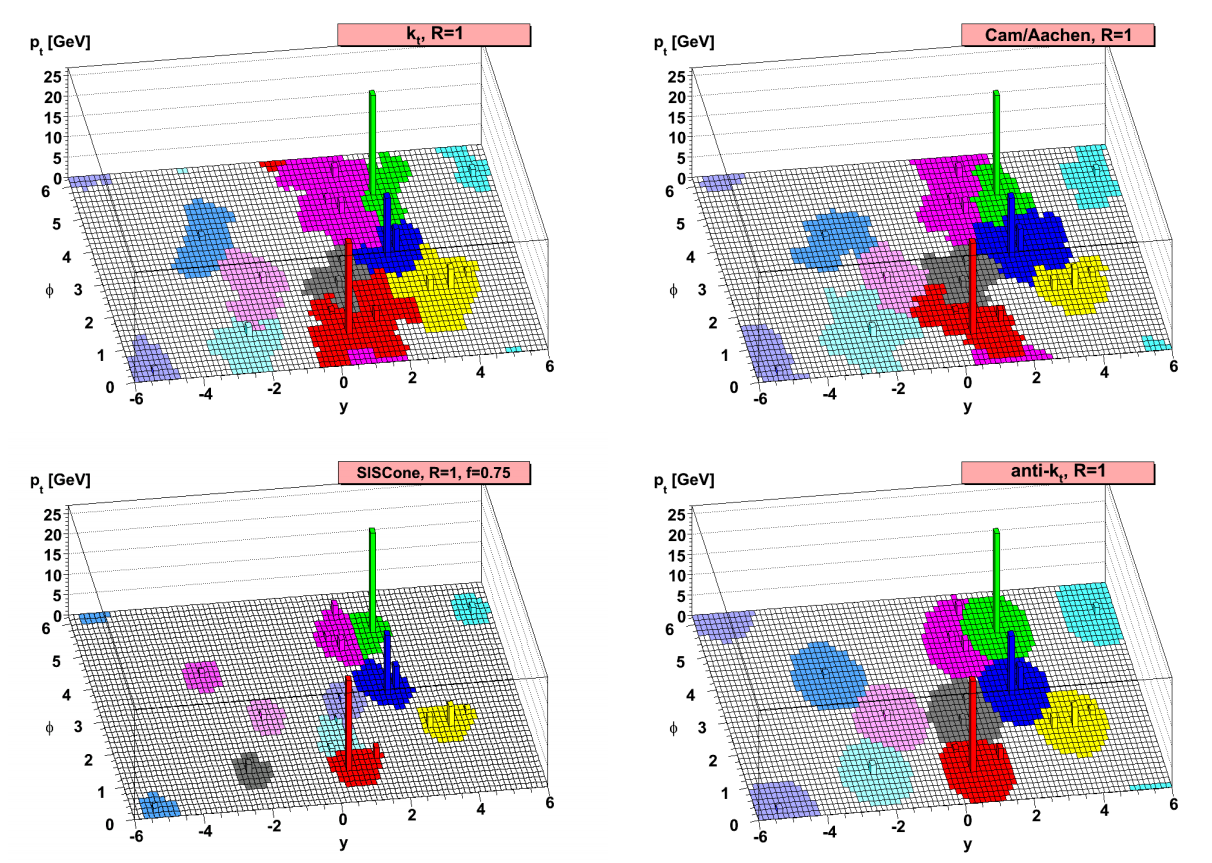
\includegraphics[width=\columnwidth]{../ThesisImages/Simulation/VarJetAlgs.png}
	\caption[A sample parton-level event with many random soft jet objects, clustered with four different jets algorithms, illustrating the areas of the resulting hard jets. For kt and Cambridge/Aachen the detailed shapes are in part determined by the specific set of ghosts used, and change when the ghosts are modified]{A sample parton-level event with many random soft jet objects, clustered with four different jets algorithms, illustrating the areas of the resulting hard jets. For kt and Cambridge/Aachen the detailed shapes are in part determined by the specific set of ghosts used, and change when the ghosts are modified \cite{antikt} 
	}
	\label{fig:VarJetAlgs}
\end{figure}

The jets in this analysis use the anti-$k_T$ algorithm \cite{antikt} with a radius parameter $R=0.4$.  Jets are not physical objects but collections of clustered particles so how they are defined can change the physics objects that are eventually analyzed.  The anti-$k_T$ algorithm is preferred because it is infrared and collinear safe.  Infrared safe jet algorithms do not merge two jets with a soft emission between them.  Adding or removing a soft term between two jets should not change which objects are called jets.  Collinear safe jet algorithms do not change the jet collection if the high transverse momentum particles is split or merged .  Another added benefit of the anti-$k_T$ jet finding algorithm is that it produces roughly circular jet objects, thereby simplifying the calculation of the energy density and simplifying the calibration of the jet object.

The anti=$k_T$ algorithm calculates the distance between an object $i$ and all possible jet objects $j$ ($d_{ij}$) and the beam ($d_{iB}$)
\[ d_{ij} = \text{min}(k_{ti}^{2p},k_{tj}^{2p})\frac{\Delta^2_{ij}}{R},\qquad 
d_{iB} = k_{ti}^{2p} \] 
where $k_{ti}$ is the transverse momentum, $\Delta$ is the distance between the objects, and $p=-1$.  This is a general form for the type of algorithm where the inclusive $k_T$ algorithm has a p value of 1 and the inclusive Cambridge/Aachen algorithm has a p value of 0 \cite{CambridgeAachen}.  The algorithm then follows that if $d_{ij}$ is smaller than $d_{iB}$ then objects $i$ and $j$ are merged, otherwise $i$ is labeled as a jet and removed from the list of entries of possible jet objects.  This is repeated for all entries in the list of possible jet objects.

Jet cleaning is also applied to remove events with jets built from known noisy parts of the calorimeter due to particular calorimeter cells or non-collision background in those areas \cite{JetCleaning}.  To reduce selecting jets that originate from pileup interactions, another requirement on the jet object is made on the jet vertex tagger \cite{JetJVT, JetCleanTwiki} as follows:
\begin{enumerate}
\item For jets with $20 \mathrm{ GeV } < p_{T} < 60 \mathrm{ GeV }$ and $|\eta| < 2.4$: if any jet is bad AND that jet is not marked as pileup by JVT, then reject the event
\item For jets with $20 \mathrm{ GeV } < p_{T} < 60 \mathrm{ GeV }$ and $|\eta| \geq 2.4$: if any jet is bad, then reject the event
\item For jets with $p_{T} \geq 60 \mathrm{ GeV }$: if any jet is bad, then reject the event
\end{enumerate}


\subsubsection{B-Jets}

While jets originate from any quark, jets coming from b quarks can be identified due to their decay products.  B quarks hadronize into b-hadrons which have a relatively long lifetime compared to many other hadrons produced from light quarks.  The longer lifetime and the relativistic speeds at which the hadrons travel mean the particle travels a measureable distance before it decays ($400-500 \mu m$)\cite{CMSct}.  Thus, the vertex reconstructed from the energy coming from a b hadron decay can be traced back to a point that does not correspond to the primary vertex of the event.    A pictoral representation of a b quark decay is shown in Figure \ref{fig:BTagVars}.  The b-jet vertex is called the secondary vertex.  

\begin{figure}[h!]
	\centering
	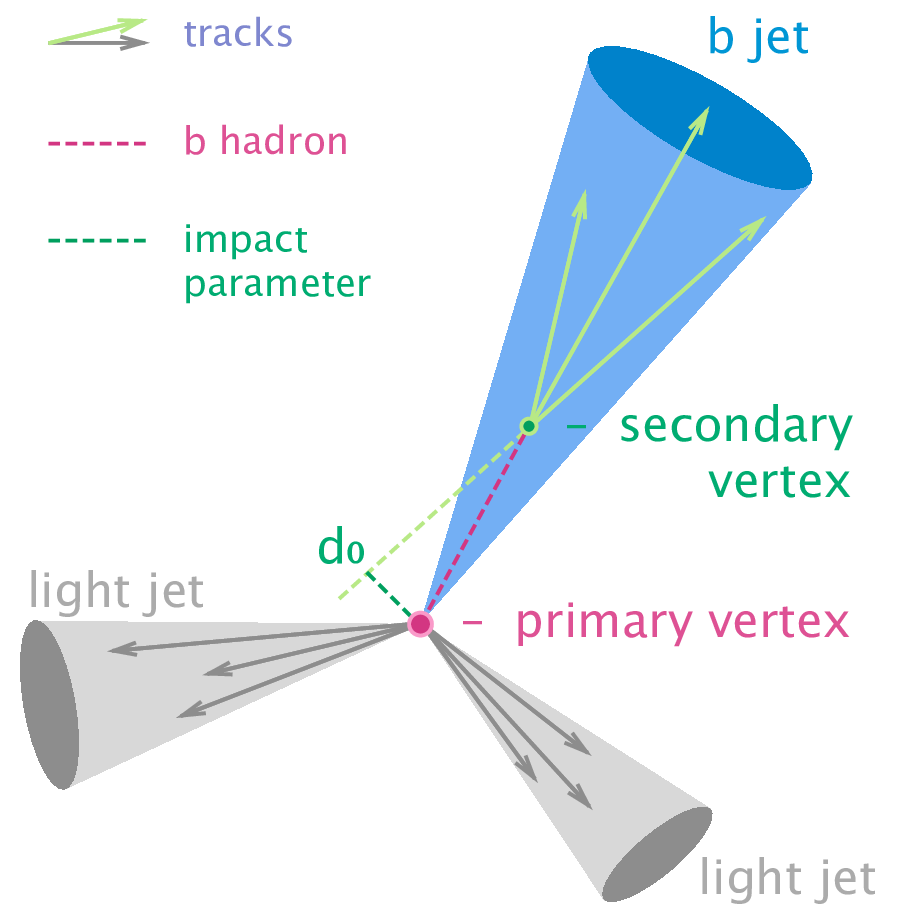
\includegraphics[width=.5\columnwidth]{../ThesisImages/Simulation/B-tagging_diagram.png}
	\caption[Pictoral representation of an event with a b-jet showing the secondary vertex and impact parameter]{Pictoral representation of an event with a b-jet showing the secondary vertex and impact parameter \cite{BTagImg} 
	}
	\label{fig:BTagVars}
\end{figure}

In addition to the secondary vertex, other variables are helpful in identifiying jets coming from b quarks.  By back tracing the tracks within the displaced vertex the minimum distance between the track and the interaction point can be measured, known as the impact parameter.  Reconstructing the decay chain of the jet is also used in determining the providence of the jet.  This information is used in a multivariate analysis (MVA) to identify jets coming from b quarks and reject jets coming from light quarks.

The MVA used in this analysis is the MV2c10, the discriminant used for b-jet identification \cite{BJet1718}.  The output distributions for various flavors of jets as well as background rejection and signal efficiency plots are shown in Figure \ref{fig:BTag}.  The c10 in the algorithm name refers to the background training sample of the MVA consisting of a 10\% fraction of c-jets.  The 77\% efficiency fixed-cut working point for b-jet identification was chosen for this analysis, discussed in Section \ref{sec:NN}.  Differences in efficiency of b-tagging between data and simulation is taken into account with working point specific scale factors provided by the ATLAS Flavour Tagging Combined Performance group.

\begin{figure}[h!]
	\centering
	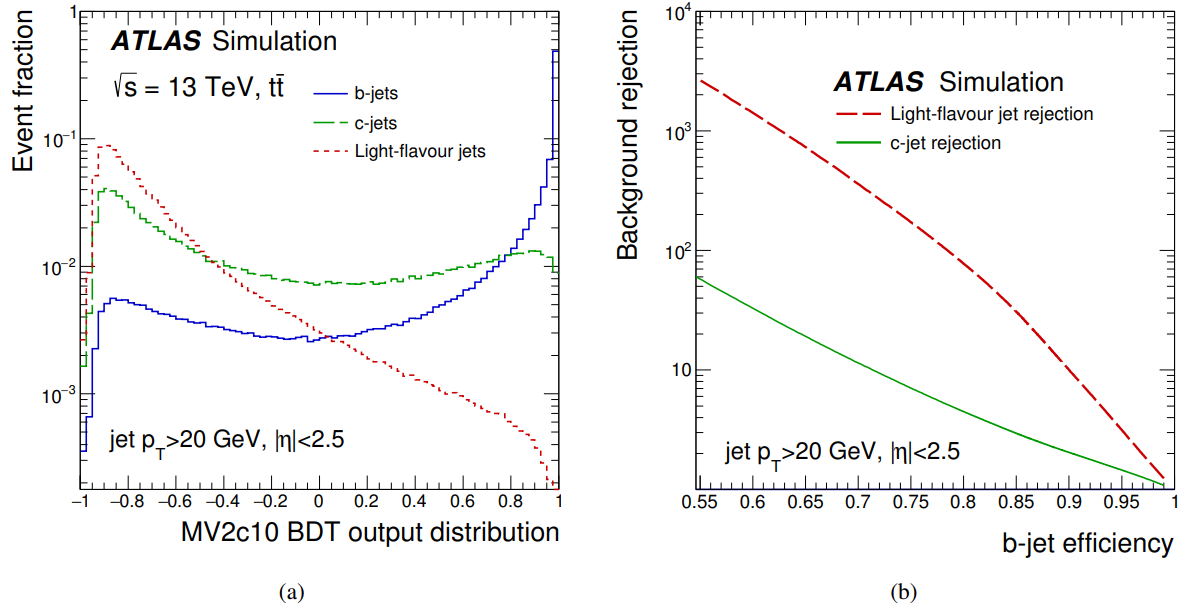
\includegraphics[width=\columnwidth]{../ThesisImages/Simulation/BTagMV2c10andRejVsEff.png}
	\caption[The MV2c10 output for b, c, and light flavored jets in simulated $t\bar{t}$ and the background rejection as a function of the b-jet efficiency]{The MV2c10 output for b, c, and light flavored jets in simulated $t\bar{t}$ and the background rejection as a function of the b-jet efficiency \cite{BJetMVA}
	}
	\label{fig:BTag}
\end{figure}


%\cite{Takubo:2017wvt}%IBL Preformance
\label{sec:bjetReco}

\subsection{Missing Transverse Energy}
The remaining signal object that has yet to be discussed is the neutrino coming from the W boson decay.  Neutrinos do not interact with the detectors as they pass through the ATLAS detector.  The only way to measure any properties of the neutrino in ATLAS events is to use conservation of momentum.  As previously mentioned the collision energy is unknown as partons do not carry a consistent fraction of the beam proton energy.  However, in the transverse plane to the beamline the total momentum is known to be very small.  Before the collision there is on the order of 1 GeV of momentum in the transverse plane.  Therefore, the total transverse momentum of the collision products should be approximately zero.

Any imbalance in the momentum is referred to as Missing Transverse Momentum ($\slashed{E}_T$).  The negative vector sum of all reconstructed objects plus an additional soft term are used to calculate the missing energy in the x-plane and the y-plane\cite{METreco}.  A magnitude and an aziumuthal angle are calculated to give the \textbf{$\slashed{E}_T$} vector in the transverse plane but this does not directly correspond to a neutrino which also has a momentum in the z direction.

\subsubsection{Neutrino Reconstruction}
In this analysis the signal contains only one source of missing energy, therefore all of the missing energy can be used to reconstruct a neturino object.  There is an ambiguity in the choice of the neutrino z-momentum.  To find the z-momentum a $\chi^2$ minimization is done:
\[ \chi^2 = \chi_{\text{SMTop}}^2 + \chi_{\text{W}}^2 \]
\[ \chi^2 = \frac{(m_{\text{bjet},l,\nu}-m_t)^2}{\sigma_{\text{SMTop}}^2} + \frac{(m_{l,\nu}-m_W)^2}{\sigma_W^2} \]
The widths $sigma_{\text{SMTop}}$ and $\sigma_W^2$ are determined from signal Monte Carlo.  The event objects are combined to calculate the invariant mass of the top quark (the combination of the b-jet, lepton, and neutrino) and the W boson (combination of the lepton and neutrino).  The $\chi^2$ minimization is is done while varying the z-momentum of the neturino.  The neutrino momentum that corresponds to the smallest $\chi^2$ value is given assigned to the neutrino object for further use in the analysis.  The $\chi^2$ values are also used as a discriminating variable and fed into a neural network (Section \ref{sec:NN}).

\subsection{Overlap Removal}
\label{sec:OverlapRemoval}
Tracks and energy deposits within the detector can, in some cases, be used to reconstruct multiple objects.  To prevent using these tracks and deposits multiple times a standard overlap removal procedure is applied to objects.  First, electrons that share tracks with any other electrons are removed.  Any electron sharing a track with a muon is then also removed.  Any jet that is found within  $\Delta R < 0.2$ of an electron is removed.  Then any jet with less than 3 tracks associated with it within $\Delta R < 0.2$ of a muon object is removed.  After that any muon found withing $\Delta R < 0.4$ of a jet is removed and any photon within $\Delta R < 0.4$ of an electron or muon object is removed. % Any jet found within $\Delta R < 0.4$ of a \textit{Loose} photon is also removed. 

\subsection{Duplicate Event Removal}
As specialized higher statistic samples are used for processes with prompt photons a double counting of events could occur with the nominal MC samples.  For example, in addition to the $t\bar{t}$ sample a sample of $t\bar{t}+\gamma$ events are used.  This is true for the W+jets/Z+jets and special samples of W+jets+$\gamma$ and Z+jets+$\gamma$.  Therefore a truth based matching scheme is used to remove events in the nominal samples that match with the photon types produced in the specialized $+\gamma$ samples i.e., they contain a truth photon that does not originate from a hadron or lepton.

%-------------------------------------------------------------------------------


%-------------------------------------------------------------------------------
%\newpage
%\section{Event Selection}
%\label{sec:evsel}
\newpage
\section{Initial Event Selection}
\label{sec:InitSelec}
Initial event selection is done to ensure that events that are accepted into the analysis are not contaminated by extremely noisey detector environments and happened during times when the ATLAS detector was accepting events properly.  All of the events  have the same initial set of criteria for determining whether or not the event is looked at any further for this analysis, applying to both MC and Data.  These initial checks are as follows:

\begin{itemize}
\item Only events occuring during runs good for physics
\item Good Calorimeter status: Ensures that the LAr and Tile calorimeters are not experiencing a noise burst at the time of the event
\item Requires a primay vertex to be reconstructed for the event which ensures timing of further reconstructed objects are placed with the correct vertex
\item Global Trigger Decision: Selects events based on wheter they passed one of the triggers including the trigger thresholds, further discussion in Section \ref{sec:GTRIGDEC}
\item Trigger Match: Select events where an electron or muon matches the trigger
\item Overlap Removal as discussed in Section \ref{sec:OverlapRemoval}
\item Ignore events that have a bad muon, occurs mostly in the transition region and the cathode strip chamber regions.
\item Jet Cleaning: Removes events with jets formed from calorimeter information from sources that have nothing to do with the energy flow from the initial hard scatter interaction
\end{itemize}

These basic event selection values are applied to every event, in both MC and Data.  On top of these various kinematic cuts are added to form the additional analysis level objects and regions used in the analysis.  These additional kinematic cuts are examined more closely in Section \ref{sec:preselcuts} and in the discussion of kinematic region creation throughout the rest of the analysis e.g., Section \ref{sec:BkgEvalCRVR}.


\subsection{Triggers}
\label{sec:GTRIGDEC}
Different HLT triggers are used for data taking periods for each year of Run 2.  This analysis takes advantage of single lepton triggers for electrons and muons to dramatically reduce backgrounds due to QCD events without leptons.  

\begin{table}[]
\small
\begin{center}
{\renewcommand{\arraystretch}{1.2}
\begin{tabular}{c|c|c|c|c}
\hline
Year  &  $p_T$ threshold [GeV]   & Identification Menu & Isolation menu & L1 Seed  \\  \hline 
2015   &    $\geq 24  $ &  Medium  &  None	& L1EM20VH	\\
           &   $\geq 60   $ &   Medium  &  None	&  -	\\  
            &  $\geq 120 $ &   Loose  &    None		& -	\\ \hline 
  &   $\geq 26   $ &  Tight  &   Gradient (Loose) 	&  -	\\
2016-2018  &   $\geq 60   $ &   Medium  &  None	&  -	\\  
 &  $\geq 140 $ &   Loose  &  None	&  -	 \\ \hline     
\end{tabular}
\caption{The electron trigger requirements in the event selections}
\label{tab:ElectronTrigs}
}
\end{center}
\end{table}

\begin{table}[]
\small
\begin{center}
{\renewcommand{\arraystretch}{1.2}
\begin{tabular}{c|c|c|c|c}
\hline
Year  &  $p_T$ threshold [GeV]   & Identification Menu & Isolation menu & L1 Seed  \\  \hline 
2015   &    $\geq 20  $ & None  &  Gradient (Loose)	& L1MU15 \\
           &   $\geq 50   $ &   None  &  None	&  -	\\   \hline 
2016-2018  &   $\geq 26   $ &  None  &   Gradient (Medium) 	&  -	\\
  &   $\geq 50   $ &   None  &  None	&  -	\\ \hline   
\end{tabular}
\caption{The muon trigger requirements in the event selections}
\label{tab:MuonTrigs}
}
\end{center}
\end{table}



\subsection{Data and MC Pre-Selection Cuts}
\label{sec:preselcuts}
The Signal Region pre-selection is defined to select events that have an opportunity to enter the final search selection.  This pre-selection selects events with exactly one massive lepton, at least two jets (at least one of which is b-tagged at the 77\% working point), transverse momentum and exactly one photon such that it resembles the expected final-state toplogy for the signal.  All of the events have the same initial set of criteria for determining whether or not the event is looked at any further for this analysis, applying to both MC and Data.  These initial checks are as follows:
%% Preselection Itemization
\begin{itemize}
\item Exactly 1 lepton (electron or muon) $p_T >$ 25 GeV
\item At least two good jets ($p_T >$ 25 GeV)
\item At least one b-tag (MV2c10, 77\% Working point)
\item $\slashed{E}_T >$ 30 GeV and $m_T^W >$ 30 GeV (for events with electrons)
\item $\slashed{E}_T >$ 20 GeV and $\slashed{E}_T + m_T^W >$ 60 GeV (for events with muons)
\item Exactly 1 photon, $p_T >$ 50 GeV %%%%%%%%%%%%%%%%%%%%%%%%%%%%%%%%%% Change if change plots
\end{itemize}

These plots are also produced before additional scale factors to account for mismodelling of various processes are taken into account.  These include the fake rate scale factors for processes where a truth electron or hadron are reconstructed to a photon and scaling to account for further mismodeling based on the order of the MC events produced (leading order, next-to-leading order, etc.).  Only statistical uncertainties are shown

Signal photons, which originate from a top quark decay, are very high $p_T$ whereas background photons typically result from soft processes.  A cut on the photon candidate $p_T$ removes much of the backgrounds while keeping a majority of the signal.  The photon $p_T$ in the preselection region is shown in Figure \ref{fig:PreSelPlots1}.  
%%SR Pre Selection Plots
\begin{figure}[h!]
\centering
\subfloat[electron channel]{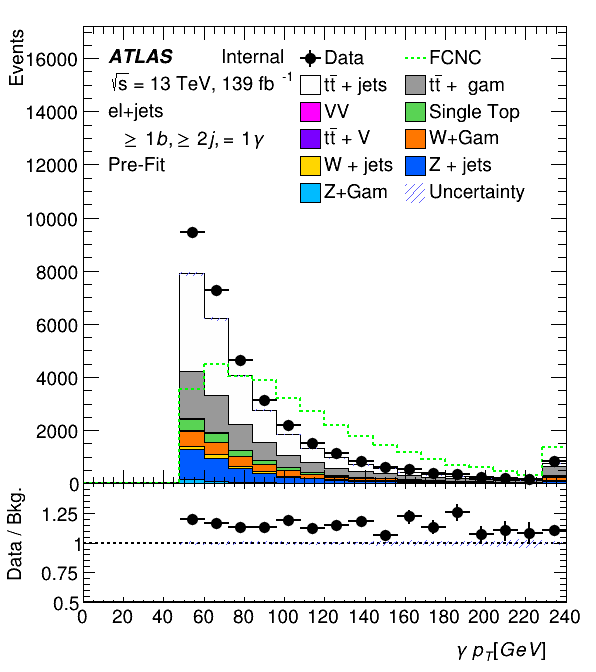
\includegraphics[width=.45\columnwidth]{../ThesisImages/RegionPlots/BeforeScaling/PreSelection/FCNC_All_ejets/Plots/PreSel_ph_pt.png}}\hfil
\subfloat[muon channel]{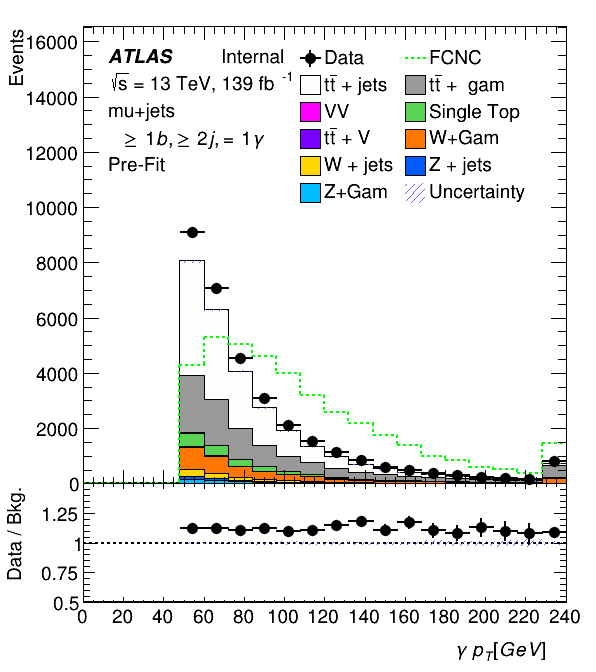
\includegraphics[width=.45\columnwidth]{../ThesisImages/RegionPlots/BeforeScaling/PreSelection/FCNC_All_mujets/Plots/PreSel_ph_pt.png}}
\caption{Photon $p_T$ in the signal region pre-preselection region.  FCNC signal branching ratio is scaled to 1\%.}
\label{fig:PreSelPlots1}
\end{figure}

Other variables of interest, i.e. those being used as inputs into the neural network are also showed in this section.  Figure \ref{fig:PreSelPlotsST} shows the $S_T$ and $m_T^W$ distributions.  Figure \ref{fig:PreSelTopMasses} shows the invariant mass distributions for both top quark candidates, $m_{Wb}$ and $m_{q\gamma}$.  The kinematic variables for the electron channel are shown in Figure \ref{fig:PreSelPlots2} and for the muon channel in Figure \ref{fig:PreSelPlots3}.  The neural network output of these events are shown in Figure \ref{fig:PreSelPlots5}

\begin{figure}[h!]
\centering
\subfloat[electron channel]{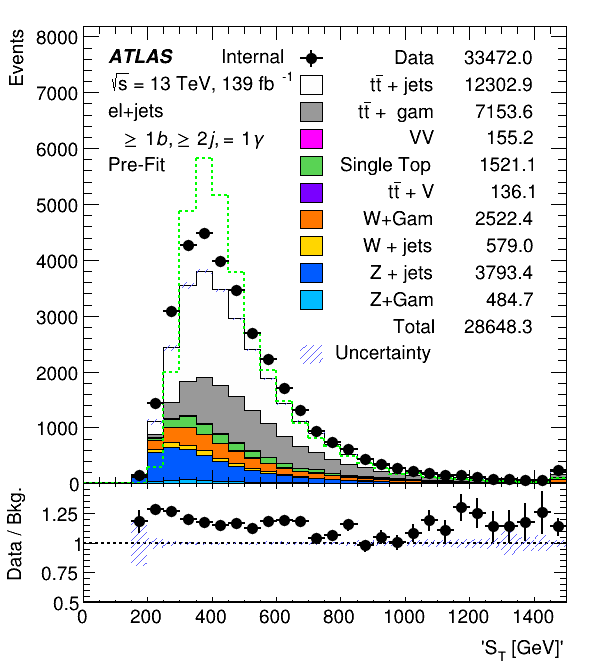
\includegraphics[width=.5\columnwidth]{../ThesisImages/RegionPlots/BeforeScaling/PreSelection/FCNC_All_ejets/Plots/PreSel_ST.png}}\hfil
\subfloat[muon channel]{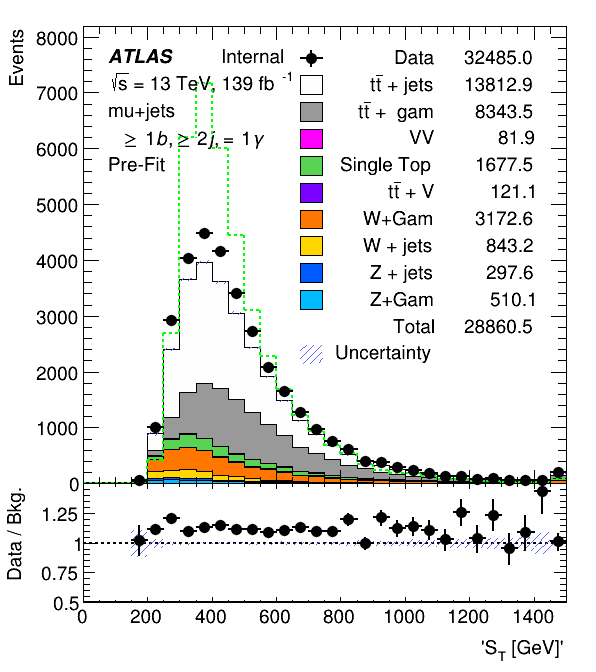
\includegraphics[width=.5\columnwidth]{../ThesisImages/RegionPlots/BeforeScaling/PreSelection/FCNC_All_mujets/Plots/PreSel_ST.png}}
\vspace{-3.mm} \setcounter{subfigure}{0}
\subfloat[electron channel]{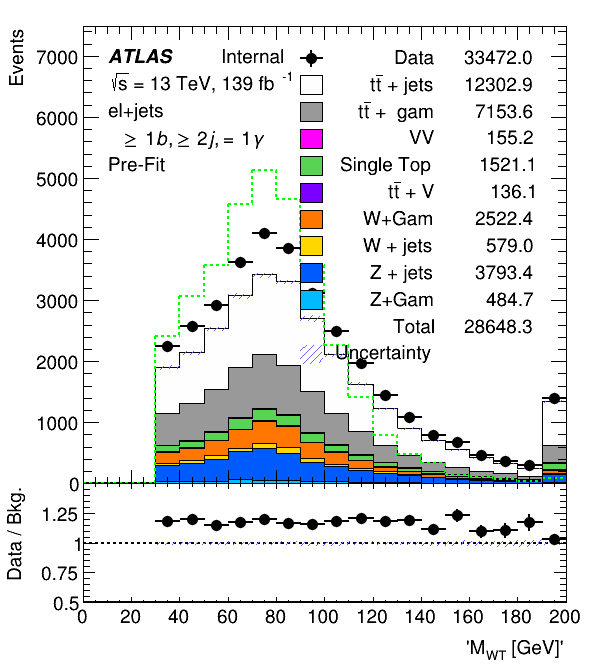
\includegraphics[width=.45\columnwidth]{../ThesisImages/RegionPlots/BeforeScaling/PreSelection/FCNC_All_ejets/Plots/PreSel_MWT.png}}\hfil
\subfloat[muon channel]{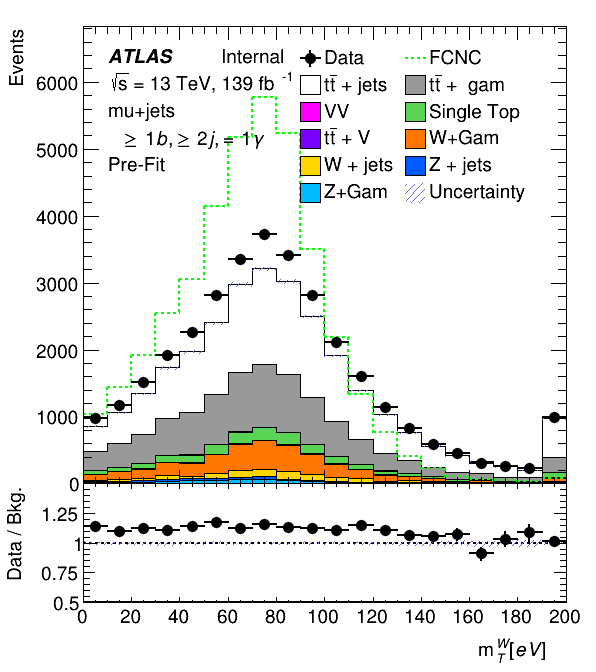
\includegraphics[width=.45\columnwidth]{../ThesisImages/RegionPlots/BeforeScaling/PreSelection/FCNC_All_mujets/Plots/PreSel_MWT.png}}
\caption{$S_T$ and $m_T^W$ in the signal region pre-selection region.  FCNC signal branching ratio is scaled to 1\%.}
\label{fig:PreSelPlotsST}
\end{figure}

\begin{figure}[h!]
\centering
\subfloat{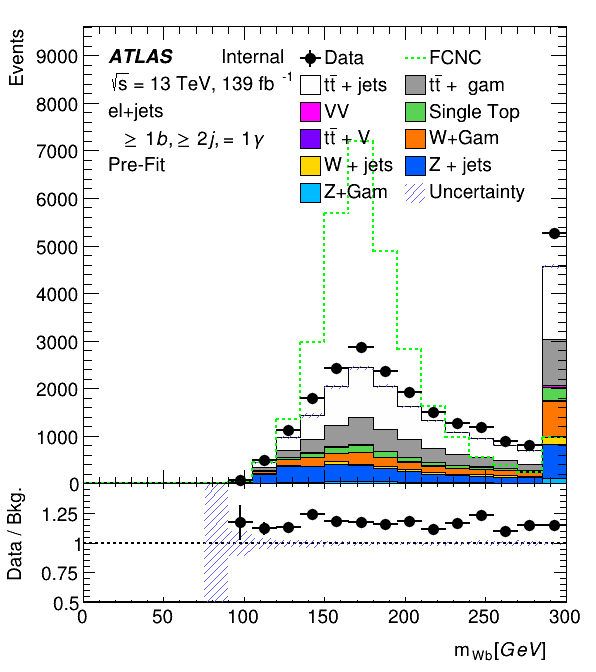
\includegraphics[width=.5\columnwidth]{../ThesisImages/RegionPlots/BeforeScaling/PreSelection/FCNC_All_ejets/Plots/PreSel_SMtop.png}}\hfil
\subfloat{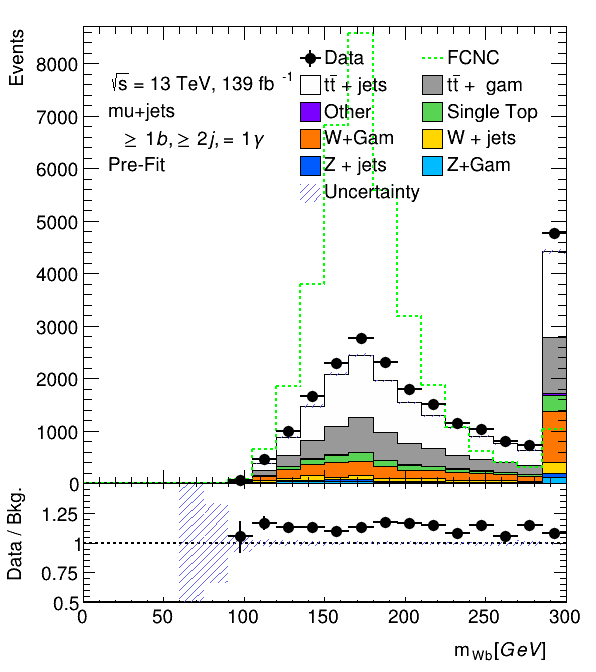
\includegraphics[width=.5\columnwidth]{../ThesisImages/RegionPlots/BeforeScaling/PreSelection/FCNC_All_mujets/Plots/PreSel_SMtop.png}}
\vspace{-3.mm} \setcounter{subfigure}{0}
\subfloat[electron channel]{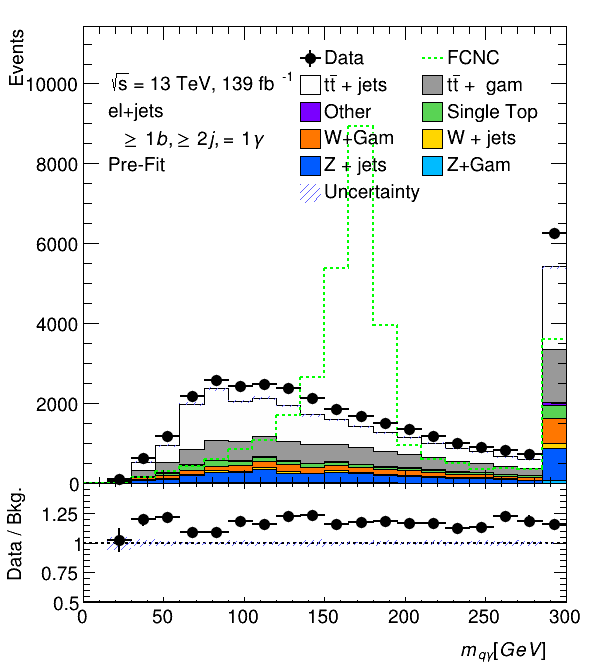
\includegraphics[width=.5\columnwidth]{../ThesisImages/RegionPlots/BeforeScaling/PreSelection/FCNC_All_ejets/Plots/PreSel_mqph.png}}\hfil
\subfloat[muon channel]{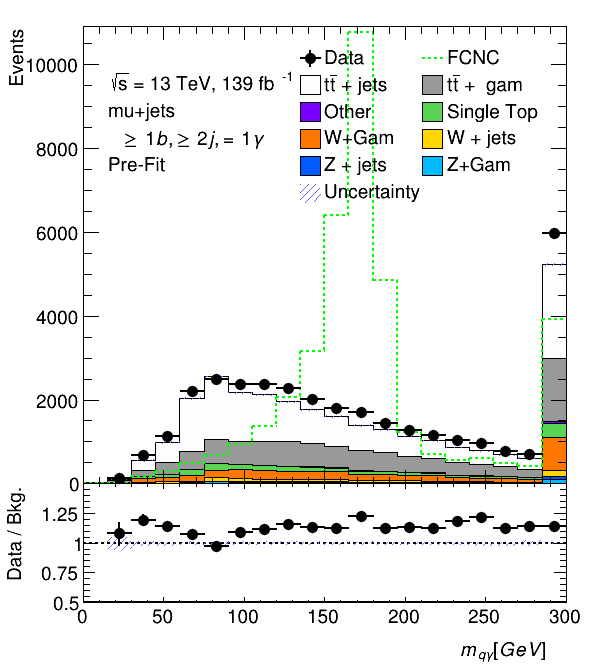
\includegraphics[width=.5\columnwidth]{../ThesisImages/RegionPlots/BeforeScaling/PreSelection/FCNC_All_mujets/Plots/PreSel_mqph.png}}
\caption{Top mass candidates in the signal region pre-selection: $m_{W b}$ and $m_{q\gamma}$. FCNC signal branching ratio is scaled to 1\%.}
\label{fig:PreSelTopMasses}
\end{figure}


%\begin{figure}[h!]
%\centering
%\subfloat{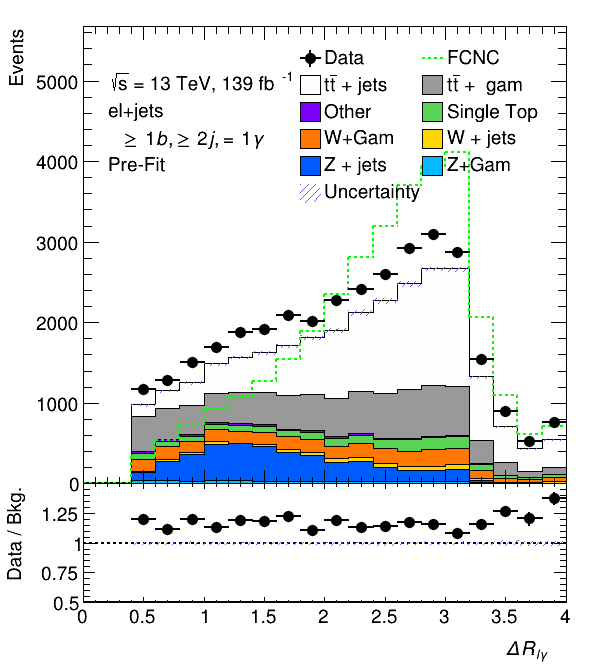
\includegraphics[width=.5\columnwidth]{../ThesisImages/RegionPlots/BeforeScaling/PreSelection/FCNC_All_ejets/Plots/PreSel_drlph.png}}\hfil
%\subfloat{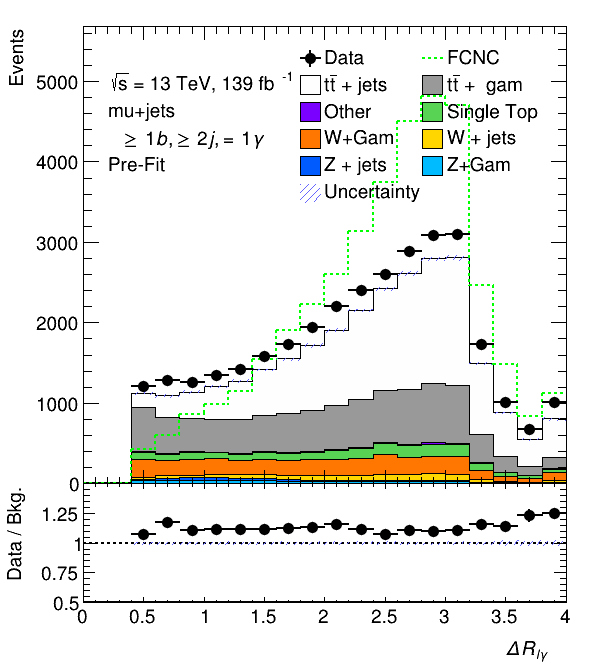
\includegraphics[width=.5\columnwidth]{../ThesisImages/RegionPlots/BeforeScaling/PreSelection/FCNC_All_mujets/Plots/PreSel_drlph.png}}
%\vspace{-3.mm} \setcounter{subfigure}{0}
%\subfloat[electron channel]{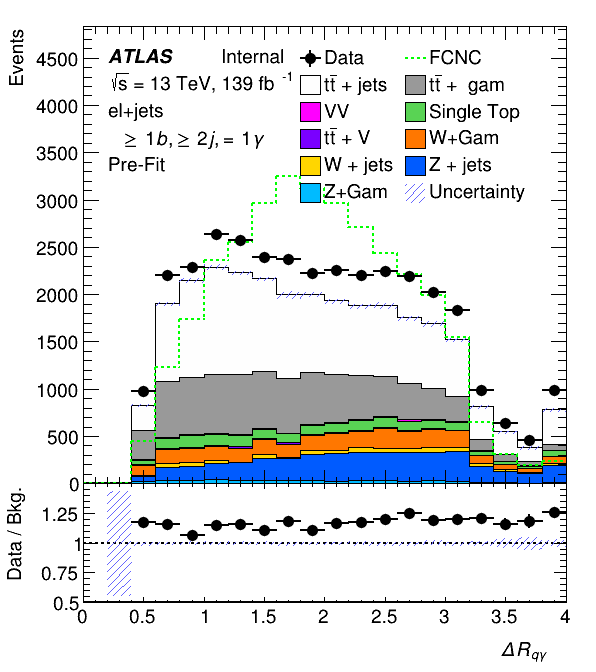
\includegraphics[width=.5\columnwidth]{../ThesisImages/RegionPlots/BeforeScaling/PreSelection/FCNC_All_ejets/Plots/PreSel_drqph.png}}\hfil
%\subfloat[muon channel]{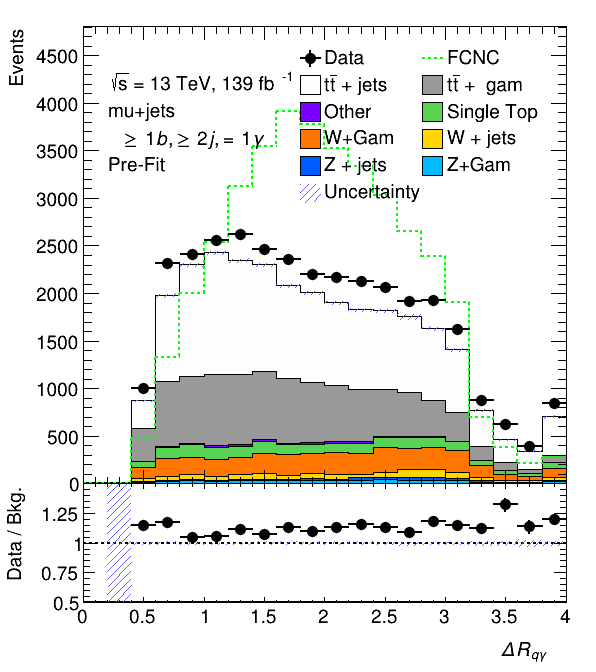
\includegraphics[width=.5\columnwidth]{../ThesisImages/RegionPlots/BeforeScaling/PreSelection/FCNC_All_mujets/Plots/PreSel_drqph.png}}
%\caption{Distance between the photon and closest light jet, $\Delta R_{l \gamma}$, and closest light jet, $\Delta R_{q\gamma}$, in the signal region pre-selection region.  FCNC signal branching ratio is scaled to 1\%}
%\label{fig:PreSeDeltaRs}
%\end{figure}


\begin{figure}[h!]
\centering
\subfloat[]{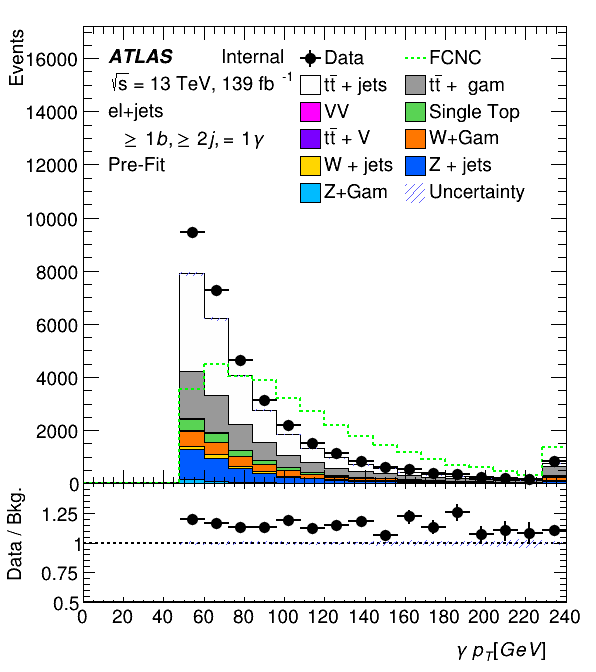
\includegraphics[width=.33\columnwidth]{../ThesisImages/RegionPlots/BeforeScaling/PreSelection/FCNC_All_ejets/Plots/PreSel_ph_pt.png}} \hfil
\subfloat[]{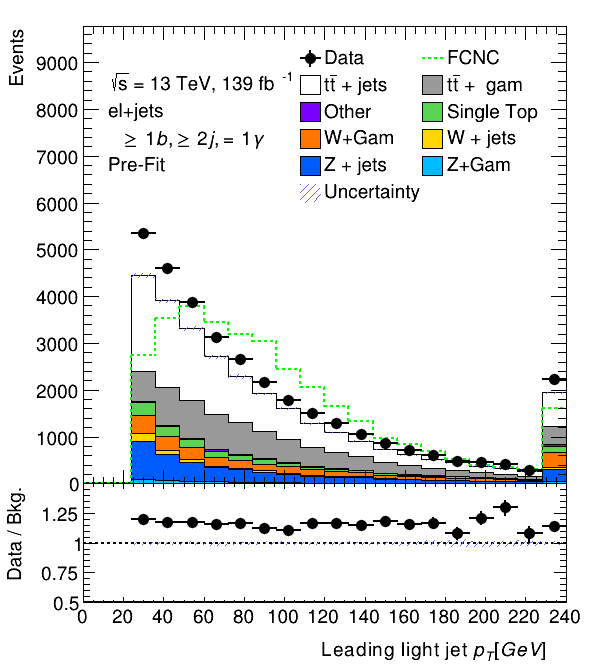
\includegraphics[width=.33\columnwidth]{../ThesisImages/RegionPlots/BeforeScaling/PreSelection/FCNC_All_ejets/Plots/PreSel_jet0_pt.png}} \hfil  
\subfloat[]{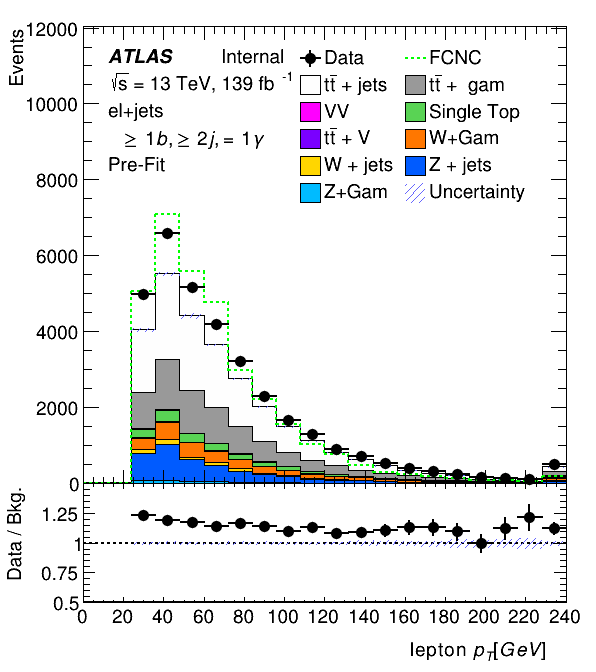
\includegraphics[width=.33\columnwidth]{../ThesisImages/RegionPlots/BeforeScaling/PreSelection/FCNC_All_ejets/Plots/PreSel_lep_pt.png}}
\vspace{-3.mm}
\subfloat[]{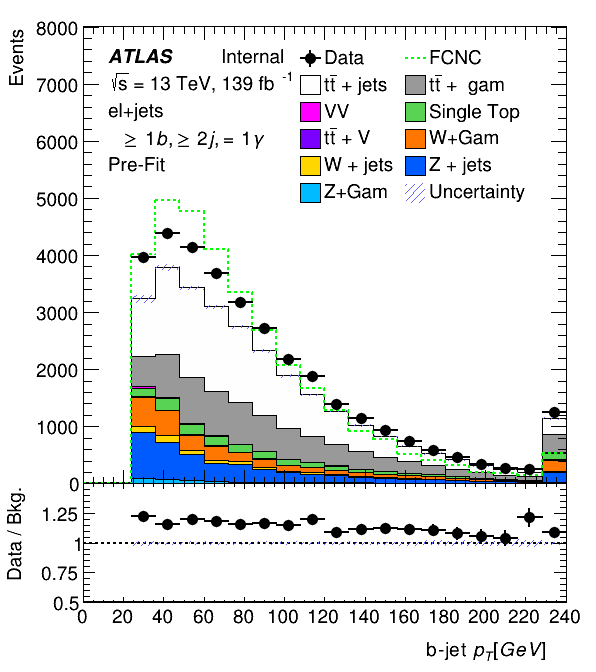
\includegraphics[width=.33\columnwidth]{../ThesisImages/RegionPlots/BeforeScaling/PreSelection/FCNC_All_ejets/Plots/PreSel_bjet0_pt.png}}\hfil
\subfloat[]{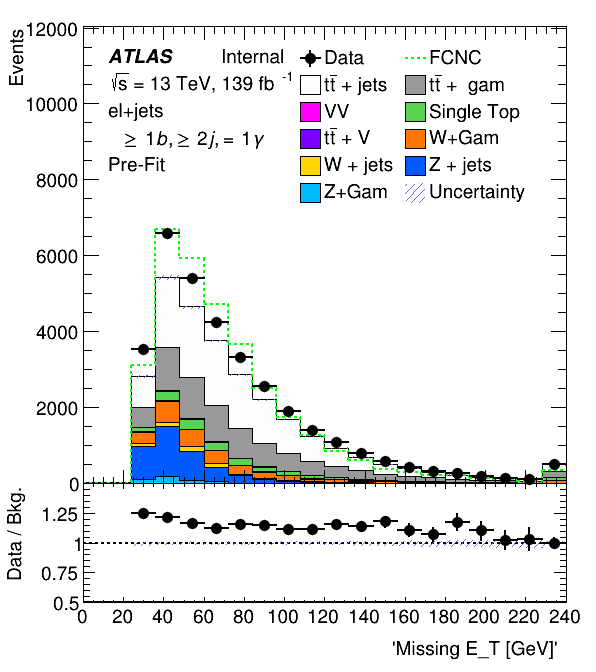
\includegraphics[width=.33\columnwidth]{../ThesisImages/RegionPlots/BeforeScaling/PreSelection/FCNC_All_ejets/Plots/PreSel_met.png}}\hfil
\subfloat[]{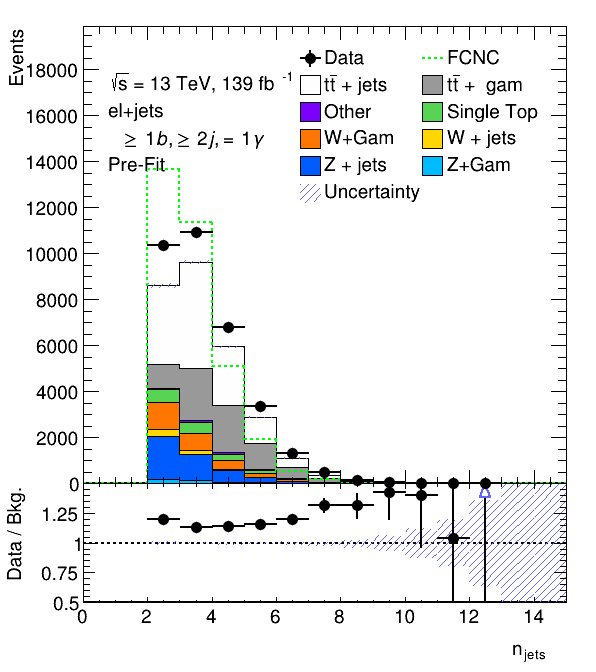
\includegraphics[width=.33\columnwidth]{../ThesisImages/RegionPlots/BeforeScaling/PreSelection/FCNC_All_ejets/Plots/PreSel_njet.png}}
\caption{Photon $p_T$ (a), leading light jet $p_T$ (b), lepton $p_T$ (c), b-jet $p_T$(d), $\slashed{E}_T$ (e), and $n_{\text{jets}}$ (f) plots in the signal region pre-selection for the electron+jets channel.  FCNC signal branching ratio is scaled to 1\%. }
\label{fig:PreSelPlots2}
\end{figure}


\begin{figure}[h!]
\centering
\subfloat[]{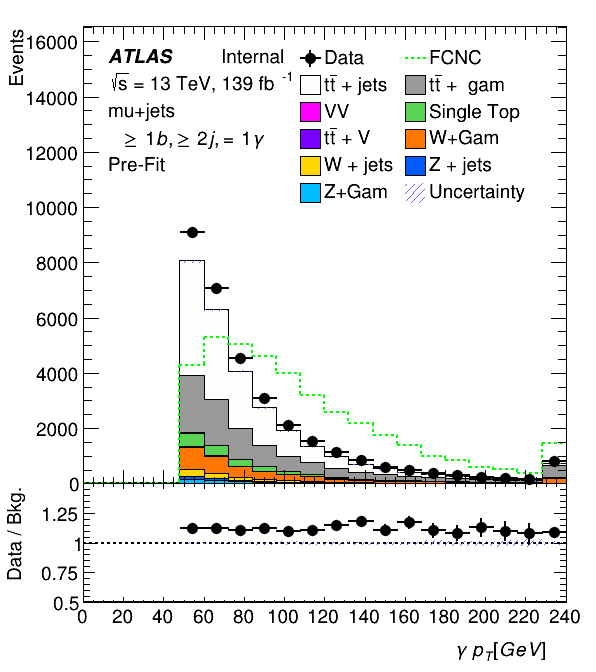
\includegraphics[width=.33\columnwidth]{../ThesisImages/RegionPlots/BeforeScaling/PreSelection/FCNC_All_mujets/Plots/PreSel_ph_pt.png}}\hfil
\subfloat[]{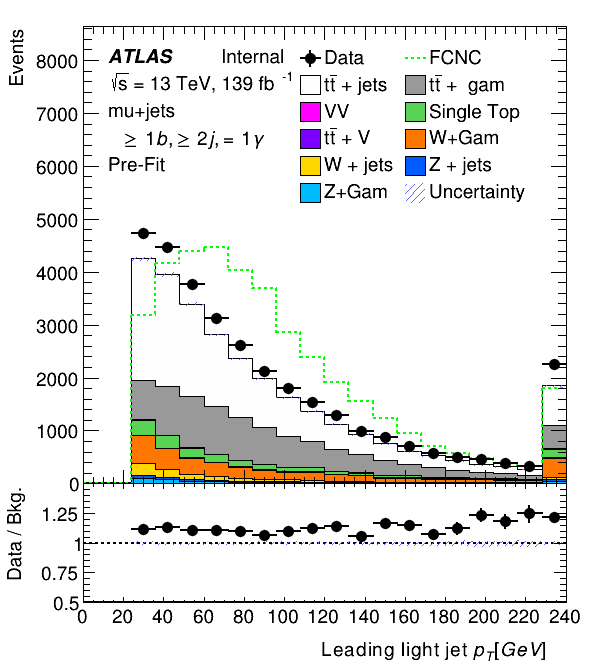
\includegraphics[width=.33\columnwidth]{../ThesisImages/RegionPlots/BeforeScaling/PreSelection/FCNC_All_mujets/Plots/PreSel_jet0_pt.png}}\hfil  
\subfloat[]{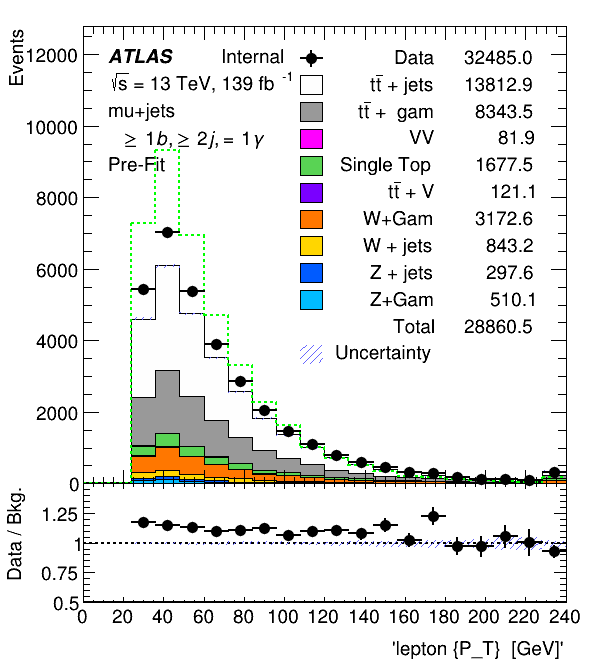
\includegraphics[width=.33\columnwidth]{../ThesisImages/RegionPlots/BeforeScaling/PreSelection/FCNC_All_mujets/Plots/PreSel_lep_pt.png}}
\vspace{-3.mm}
\subfloat[]{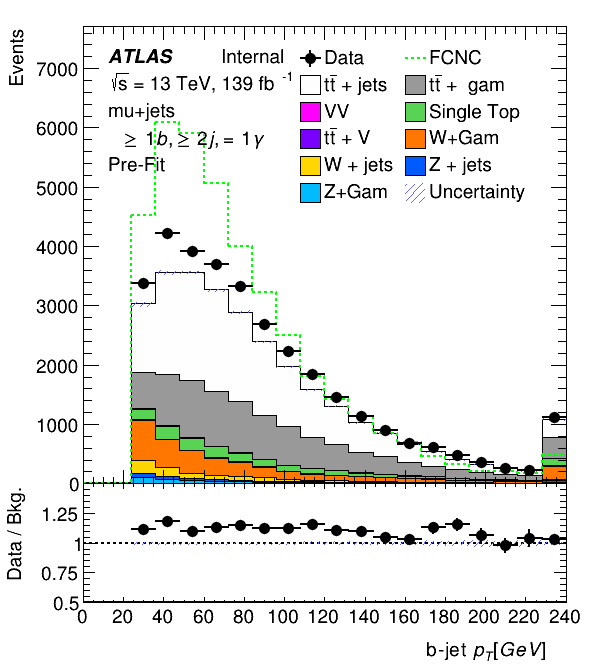
\includegraphics[width=.33\columnwidth]{../ThesisImages/RegionPlots/BeforeScaling/PreSelection/FCNC_All_mujets/Plots/PreSel_bjet0_pt.png}}\hfil
\subfloat[]{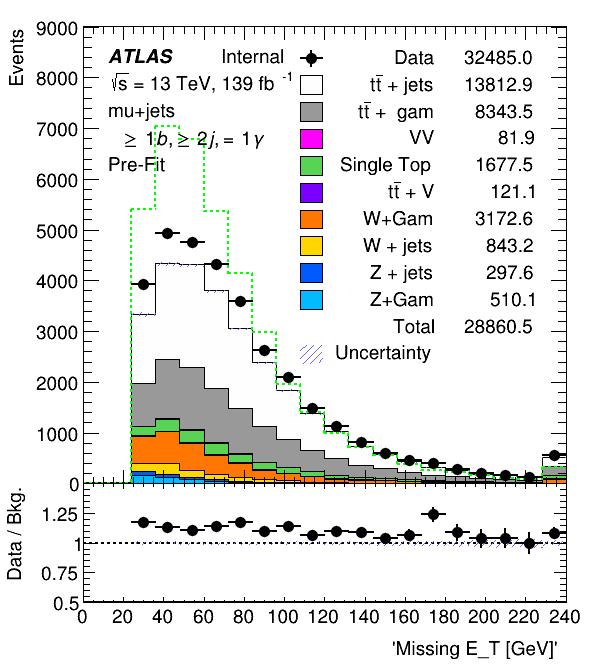
\includegraphics[width=.33\columnwidth]{../ThesisImages/RegionPlots/BeforeScaling/PreSelection/FCNC_All_mujets/Plots/PreSel_met.png}}\hfil
\subfloat[]{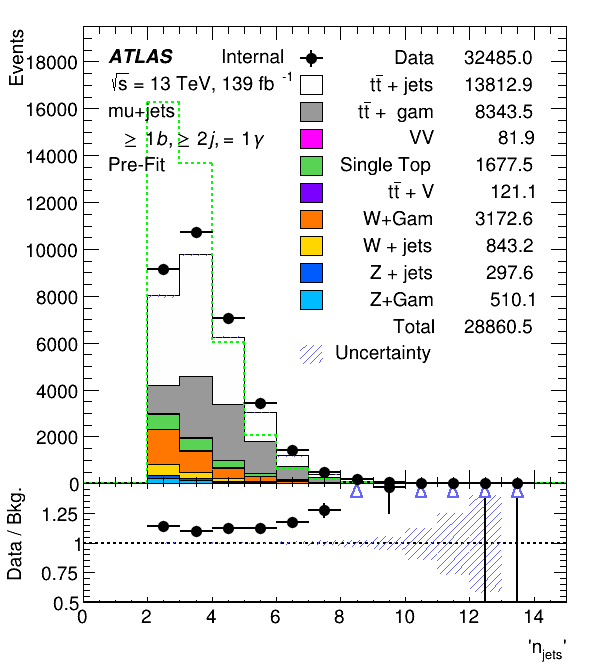
\includegraphics[width=.33\columnwidth]{../ThesisImages/RegionPlots/BeforeScaling/PreSelection/FCNC_All_mujets/Plots/PreSel_njet.png}}
\caption{Photon $p_T$ (a), leading light jet $p_T$ (b), lepton $p_T$ (c), b-jet $p_T$(d), $\slashed{E}_T$ (e), and $n_{\text{jets}}$ (f) plots in the signal region pre-selection for the muon+jets channel.  FCNC signal branching ratio is scaled to 1\%.}
\label{fig:PreSelPlots3}
\end{figure}

\begin{figure}[h!]
\centering
\subfloat[electron channel]{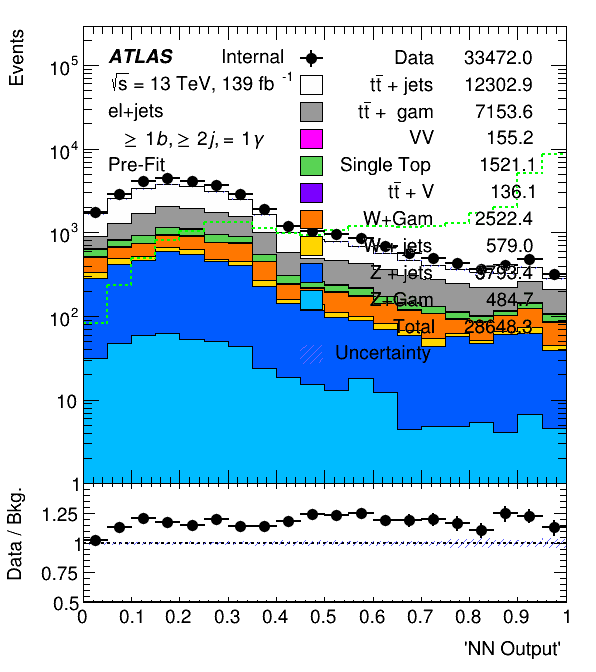
\includegraphics[width=.5\columnwidth]{../ThesisImages/RegionPlots/BeforeScaling/PreSelection/FCNC_All_ejets/Plots/PreSel_NNejet.png}}\hfil
\subfloat[muon channel]{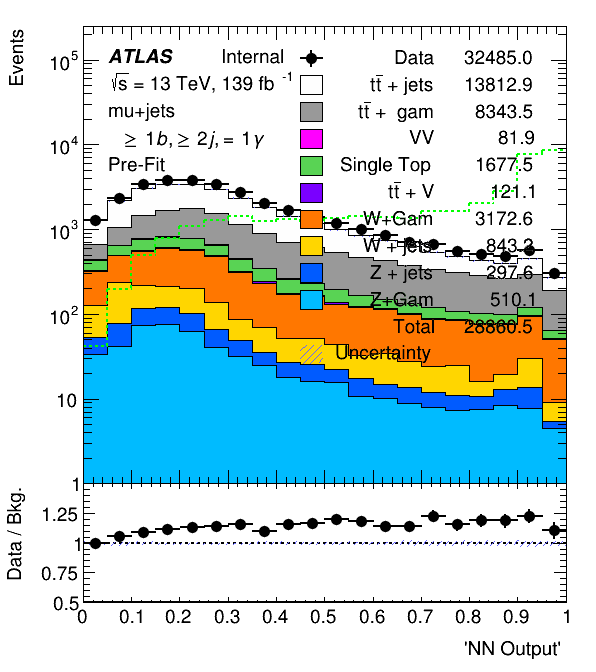
\includegraphics[width=.5\columnwidth]{../ThesisImages/RegionPlots/BeforeScaling/PreSelection/FCNC_All_mujets/Plots/PreSel_NNmujet.png}}
\caption{Output of the Neural Network in the signal region pre-selection region.  FCNC signal branching ratio is scaled to 1\%.}
\label{fig:PreSelPlots5}
\end{figure}

\subsection{Background Evaluation: Control and Validation Regions}
\label{sec:BkgEvalCRVR}
Orthogonal regions to the signal region have been created to test the preformance of Monte Carlo samples.  Control and validation regions are designed to isolate specific physics processes to determine and test the efficacy of scale factors that will be applied to the final signal region Monte Carlo evets.  These control and validation regions need to be kinematically similar to the signal region such that derived scale factors can be translated directly into the signal region and orthogonal to make sure that there is little signal contamination in the regions.  Regions have been made to test the major backgrounds expected in the signal region: $t\bar{t}$, W+jets, as well as events similar events produced with an associated photon: $t\bar{t}+\gamma$ and W+Jets+$\gamma$.  Events without real photons are described in Section \ref{sec:BKGnoPho} and regions with a real photon are described in Section \ref{sec:BKGPho}.

\subsubsection{Backgrounds Without Photons}
\label{sec:BKGnoPho}
Various background processes that do not have a real photon produced in the events can still enter the signal region if an electron or jet is mis-reconstructed as a photon.  Of these processes the largest contributors in the signal region are Standard Model $t\bar{t}$ and W+jets.  As the LHC attains higher and higher energies the QCD multijet backgrounds become increasingly hard to model due to the non-perturbative nature of the interactions.  A data-driven technique for accounting for these backgrounds is developed by scaling the major backgrounds to account for the QCD backgrounds that contribute extra jets to the major backgrounds.  Designing a single control region satisfactorily close to the signal region is impossible.  Thus, two control regions are designed, one which is W+jets rich and the other $t\bar{t}$ rich.  Scale factors for these backgrounds are derived simultaneously and tested in a third similar region for validation before being applied to other regions.  
These control and validation regions are defined as follows:
\begin{itemize}
\item All of the Initial Event Selection as outlined in Section \ref{sec:InitSelec}
\item Exactly 1 lepton (electron or muon) $p_T >$ 25 GeV
\item Number of Jets  ($p_T >$ 25 GeV) to define the regions
	\begin{itemize}
	\item Control Region 1 (W+Jets enriched): $n_{\text{jets}} = 3$
	\item Validation Region: $n_{\text{jets}} =4$
	\item Control Region 2 ($t\bar{t}$ enriched): $n_{\text{jets}} \geq 5$
	\end{itemize}
\item $\slashed{E}_T >$ 30 GeV and $m_T^W >$ 30 GeV (for events with electrons)
\item $\slashed{E}_T >$ 20 GeV and $\slashed{E}_T + m_T^W >$ 60 GeV (for events with muons)
\item Exactly 1 b-tagged jet (MV2c10, 77\% Working point)
\item 0 photons, $p_T >$ 15 GeV
\end{itemize}

\begin{figure}[h!]
\centering
\subfloat[]{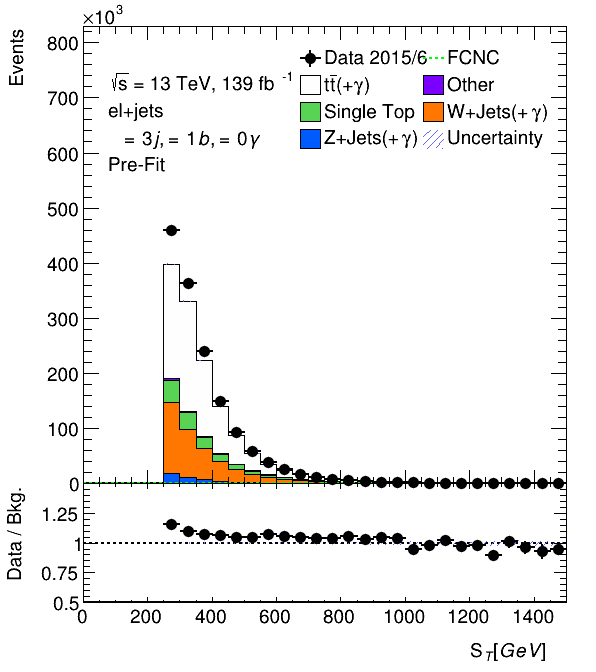
\includegraphics[width=.33\columnwidth]{../ThesisImages/RegionPlots/AfterScaling/ControlRegions/HardCodedNormFactor/FCNC_All_ejets/Plots/CR1_ST.png}}\hfil
\subfloat[]{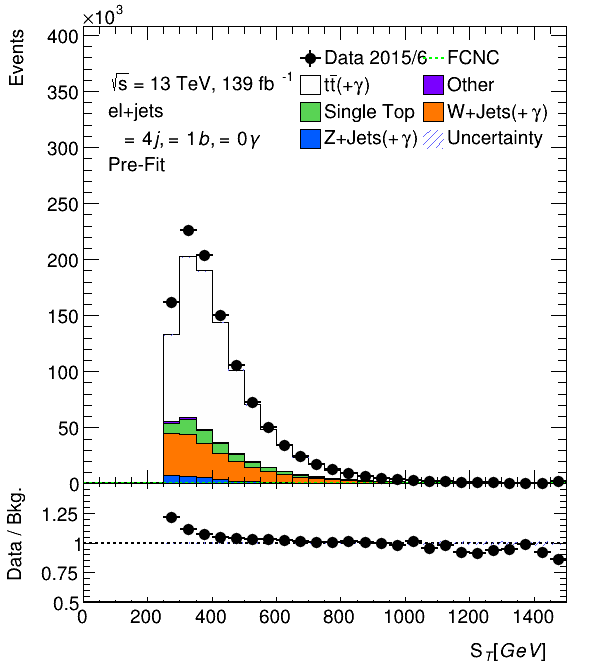
\includegraphics[width=.33\columnwidth]{../ThesisImages/RegionPlots/AfterScaling/ControlRegions/HardCodedNormFactor/FCNC_All_ejets/Plots/VR3_ST.png}}\hfil  
\subfloat[]{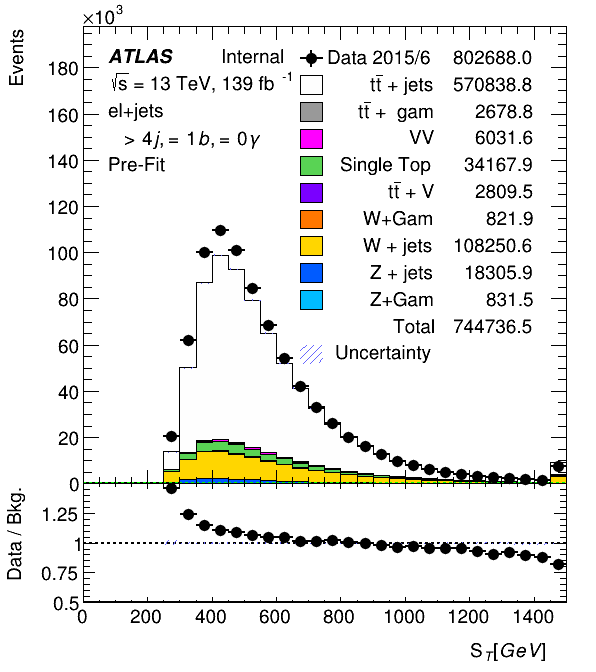
\includegraphics[width=.33\columnwidth]{../ThesisImages/RegionPlots/AfterScaling/ControlRegions/HardCodedNormFactor/FCNC_All_ejets/Plots/CR2_ST.png}}
\vspace{-3.mm}
\subfloat[]{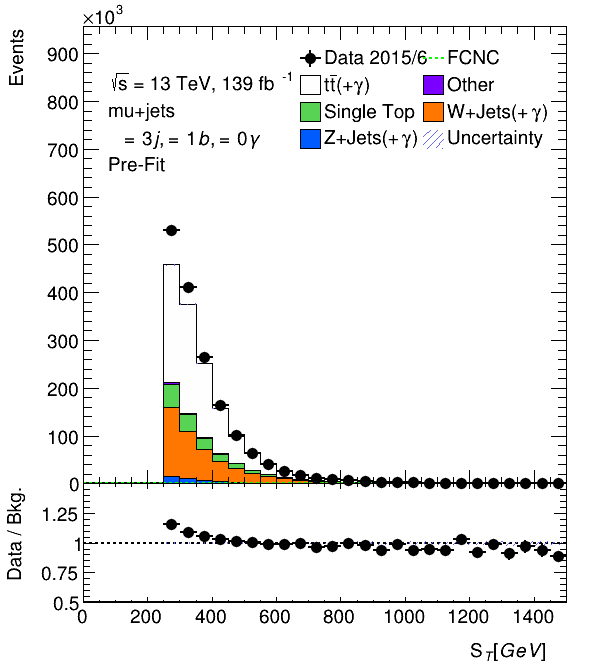
\includegraphics[width=.33\columnwidth]{../ThesisImages/RegionPlots/AfterScaling/ControlRegions/HardCodedNormFactor/FCNC_All_mujets/Plots/CR1_ST.png}}\hfil
\subfloat[]{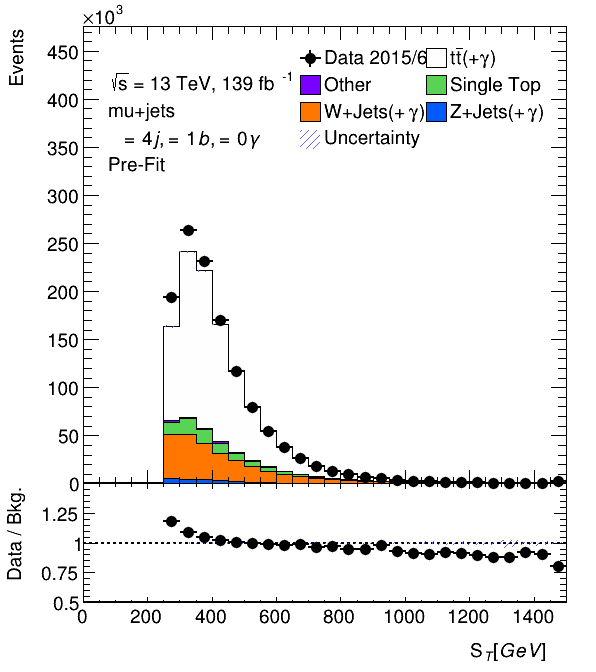
\includegraphics[width=.33\columnwidth]{../ThesisImages/RegionPlots/AfterScaling/ControlRegions/HardCodedNormFactor/FCNC_All_mujets/Plots/VR3_ST.png}}\hfil   %Change from ST Distributions to something at looks more reasonable?
\subfloat[]{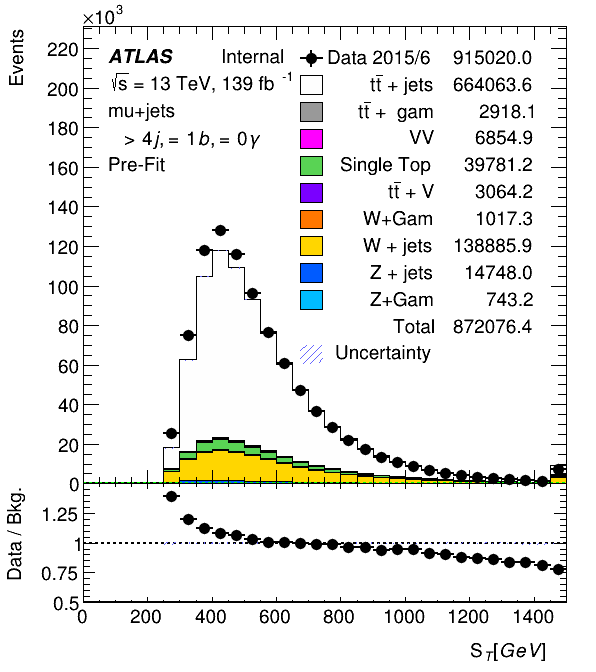
\includegraphics[width=.33\columnwidth]{../ThesisImages/RegionPlots/AfterScaling/ControlRegions/HardCodedNormFactor/FCNC_All_mujets/Plots/CR2_ST.png}}
\caption{$S_T$ distributions in the 3(a,d), 4(b,e), and 5+(c,f) jets control and validation regions. Electron channel is shown on the top and the muon channel on the bottom, before scale factors are determined.}
\label{fig:CRSTs}
\end{figure}

The efficiency of scale factors derived using control regions 1 ($n_{\text{jets}}$=3) and 2 ($n_{\text{jets}}\geq$5) are then tested in the validation region ($n_{\text{jets}}$=4).  The scale factors for the $t\bar{t}$ and W+jets MC are derived using:
\[ 
\begin{bmatrix}  
N(W)_{3j} & N(t\bar{t})_{3j} \\ N(W)_{5+j} & N(t\bar{t})_{5+j} \end{bmatrix} \begin{bmatrix} W_{SF} \\ t\bar{t}_{SF} \end{bmatrix} =
 \begin{bmatrix} N(\text{data-bkg})_{3j} \\N(\text{data-bkg})_{5j} \end{bmatrix}
\]
Figure \ref{fig:CRSTs} shows the $S_T$ distribution in both electron and muon channels before scale factors are calculated for all three kinematically separate regions.  The large mismodelling occurs at low $S_T$ values as expected as QCD processes will typically add low energy jets to the events.  The  Figures \ref{fig:VR3ejpostscale}(electron channel) and \ref{fig:VR3mujpostscale}(muon channel) show various event-level variable plots for the validation region after the scale factors have been applied.

The derived scale factors using these regions are shown in Table \ref{tab:CR12SFs}
\begin{table}[h]
\begin{center}
{\renewcommand{\arraystretch}{1.2}
\begin{tabular}{ccc}
\hline
Sample     &  e+jets SF   & $\mu$+jets SF  \\  \hline 
W+jets    &  1.22   &  1.25	\\
$t\bar{t}$  &  1.06    &  1.01	\\ \hline
\end{tabular}
\caption{Derived $t\bar{t}$ and W+jets scale factors for QCD multijet backgrounds.  }
\label{tab:CR12SFs}
}
\end{center}
\end{table}


\begin{figure}[h!]
\centering
\subfloat[]{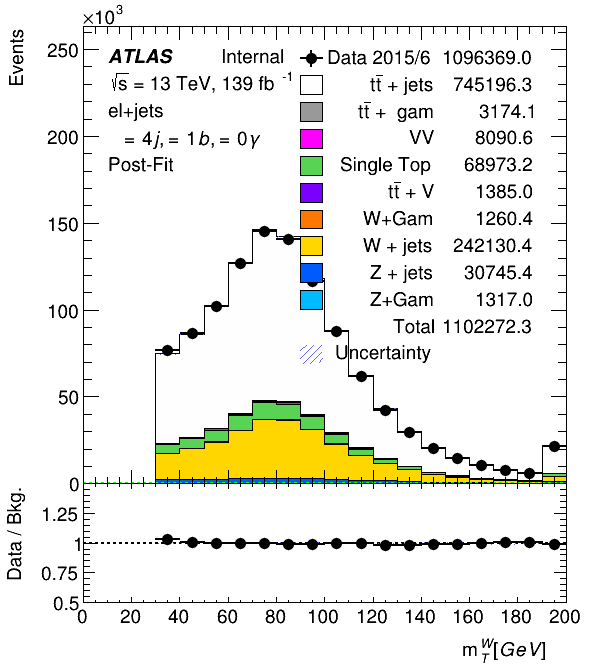
\includegraphics[width=.33\columnwidth]{../ThesisImages/RegionPlots/AfterScaling/ControlRegions/HardCodedNormFactor/FCNC_All_ejets/Plots/VR3_MWT_postFit.png}}\hfil
\subfloat[]{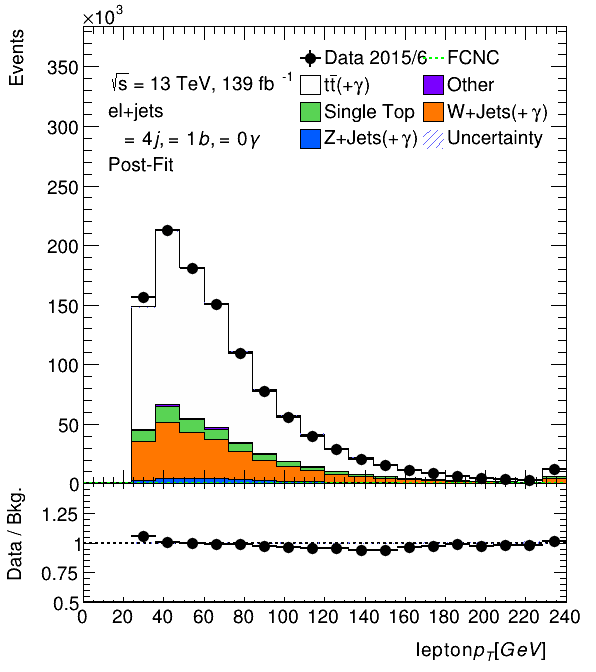
\includegraphics[width=.33\columnwidth]{../ThesisImages/RegionPlots/AfterScaling/ControlRegions/HardCodedNormFactor/FCNC_All_ejets/Plots/VR3_lep_pt_postFit.png}}\hfil  
\subfloat[]{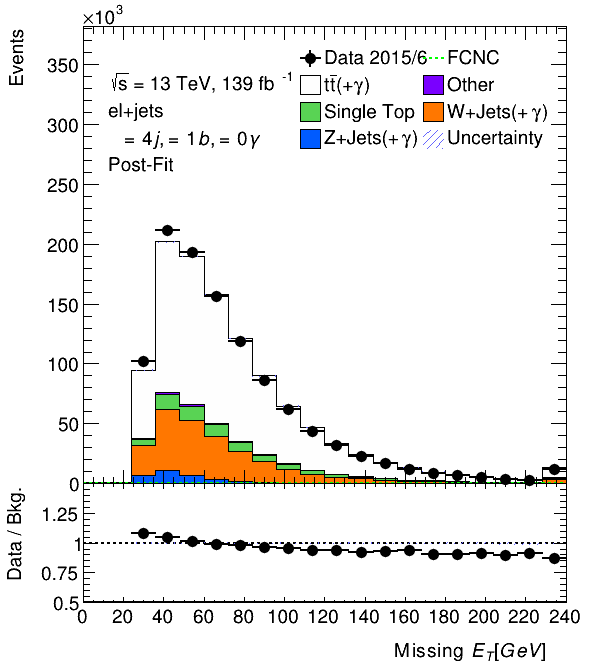
\includegraphics[width=.33\columnwidth]{../ThesisImages/RegionPlots/AfterScaling/ControlRegions/HardCodedNormFactor/FCNC_All_ejets/Plots/VR3_met_postFit.png}}
\vspace{-3.mm}
\subfloat[]{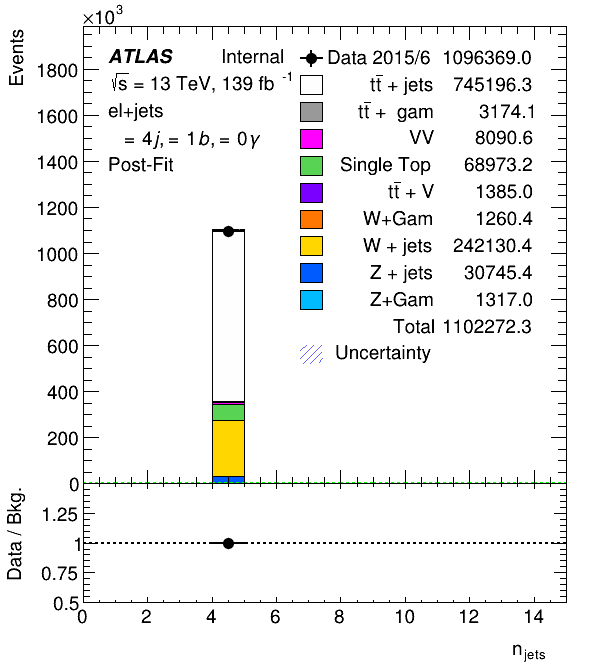
\includegraphics[width=.33\columnwidth]{../ThesisImages/RegionPlots/AfterScaling/ControlRegions/HardCodedNormFactor/FCNC_All_ejets/Plots/VR3_njet_postFit.png}}\hfil
\subfloat[]{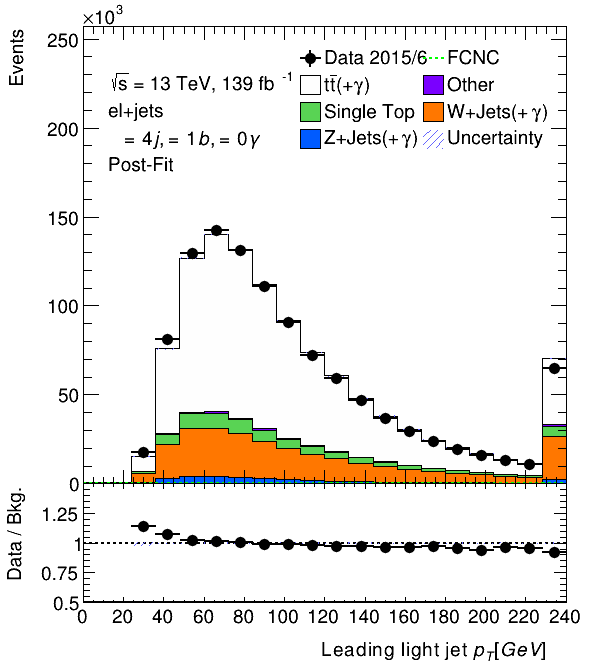
\includegraphics[width=.33\columnwidth]{../ThesisImages/RegionPlots/AfterScaling/ControlRegions/HardCodedNormFactor/FCNC_All_ejets/Plots/VR3_jet0_pt_postFit.png}}\hfil  
\subfloat[]{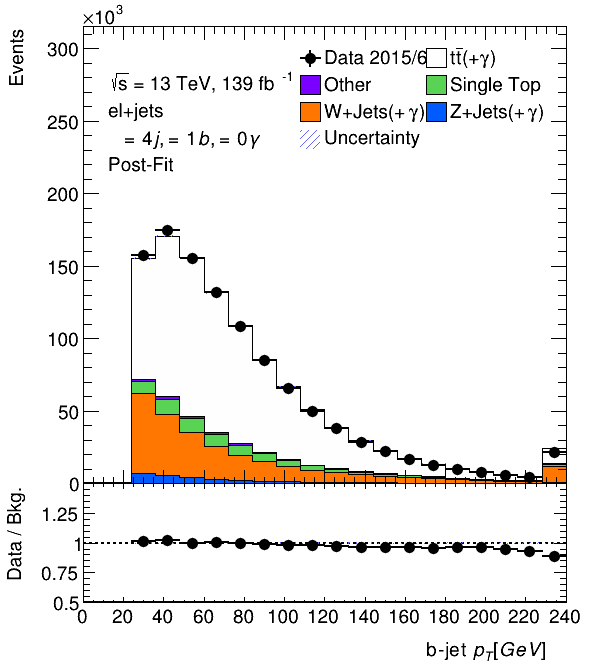
\includegraphics[width=.33\columnwidth]{../ThesisImages/RegionPlots/AfterScaling/ControlRegions/HardCodedNormFactor/FCNC_All_ejets/Plots/VR3_bjet0_pt_postFit.png}}
\caption{Event-level plots for the =4 jet validation region after scale factors have been applied in the electron channel.  FCNC signal branching ratio is scaled to 1\%.}
\label{fig:VR3ejpostscale}
\end{figure}

\begin{figure}[h!]
\centering
\subfloat[]{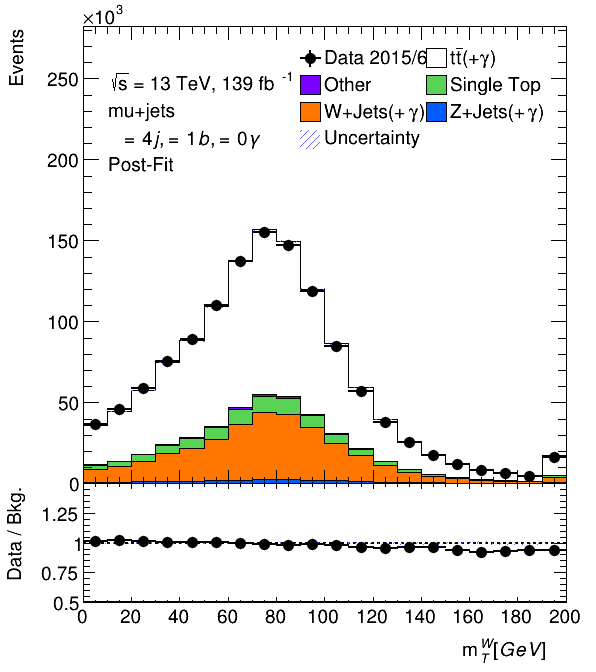
\includegraphics[width=.33\columnwidth]{../ThesisImages/RegionPlots/AfterScaling/ControlRegions/HardCodedNormFactor/FCNC_All_mujets/Plots/VR3_MWT_postFit.png}}\hfil
\subfloat[]{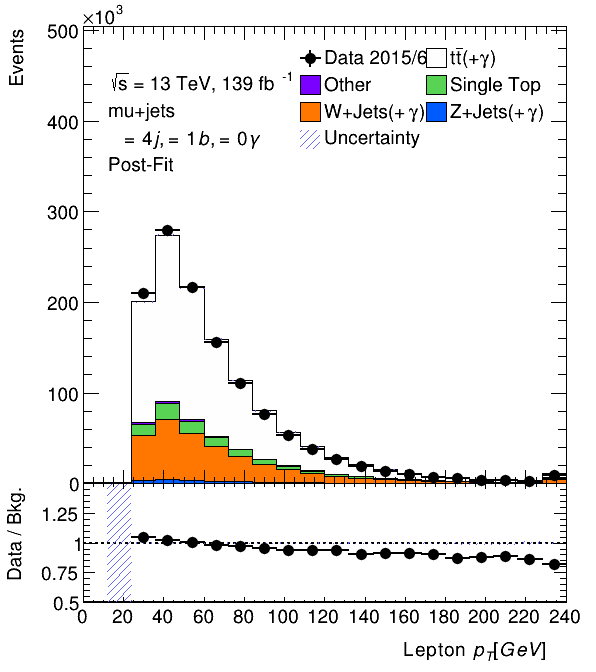
\includegraphics[width=.33\columnwidth]{../ThesisImages/RegionPlots/AfterScaling/ControlRegions/HardCodedNormFactor/FCNC_All_mujets/Plots/VR3_lep_pt_postFit.png}}\hfil 
\subfloat[]{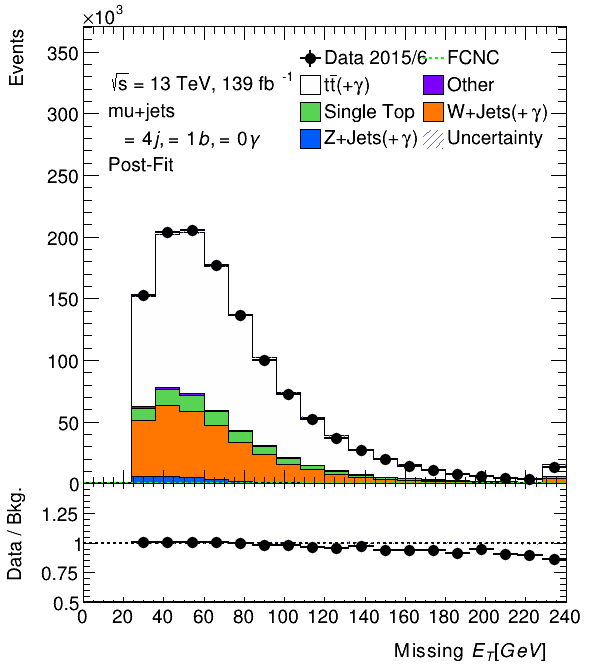
\includegraphics[width=.33\columnwidth]{../ThesisImages/RegionPlots/AfterScaling/ControlRegions/HardCodedNormFactor/FCNC_All_mujets/Plots/VR3_met_postFit.png}}
\vspace{-3.mm}
\subfloat[]{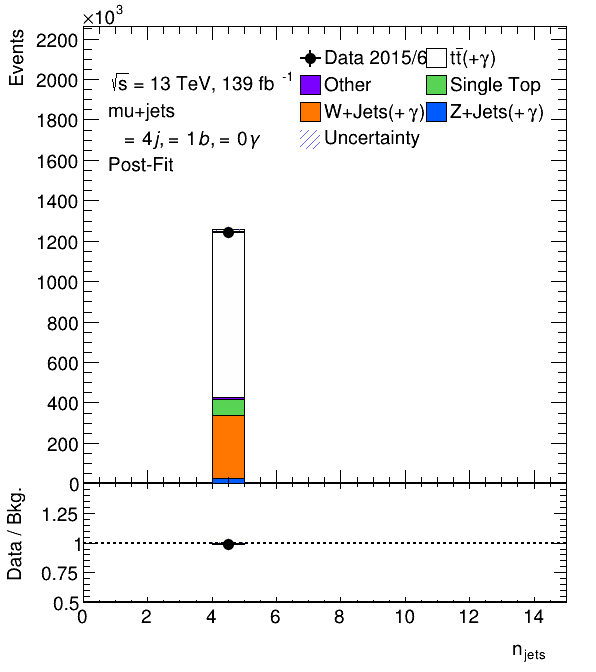
\includegraphics[width=.33\columnwidth]{../ThesisImages/RegionPlots/AfterScaling/ControlRegions/HardCodedNormFactor/FCNC_All_mujets/Plots/VR3_njet_postFit.png}}\hfil
\subfloat[]{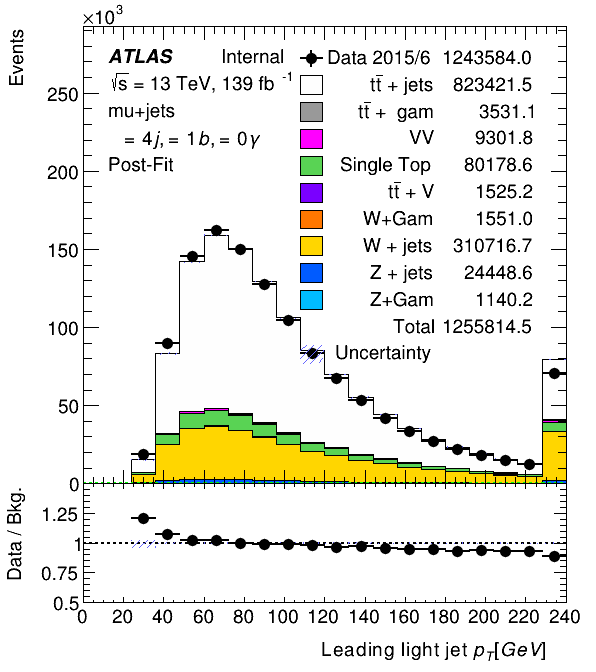
\includegraphics[width=.33\columnwidth]{../ThesisImages/RegionPlots/AfterScaling/ControlRegions/HardCodedNormFactor/FCNC_All_mujets/Plots/VR3_jet0_pt_postFit.png}}\hfil 
\subfloat[]{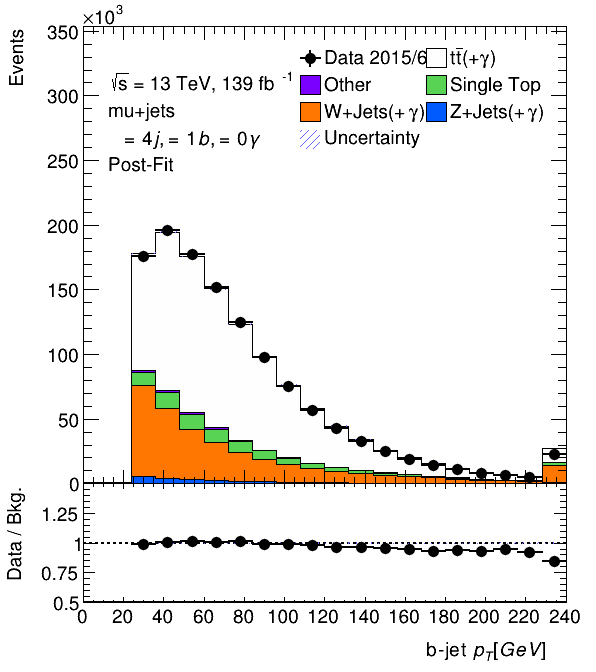
\includegraphics[width=.33\columnwidth]{../ThesisImages/RegionPlots/AfterScaling/ControlRegions/HardCodedNormFactor/FCNC_All_mujets/Plots/VR3_bjet0_pt_postFit.png}}
\caption{Event-level plots for the =4 jet validation region after scale factors have been applied in the muon channel.  FCNC signal branching ratio is scaled to 1\%.}
\label{fig:VR3mujpostscale}
\end{figure}


%%%%%%%%%%%%%%%%%%%%%%%%%%%%%%%%%%%%%%%%%%
%%%%%%%%%%%%%%%%%%%%%%%%%%%%%%%%%%%%%%%%%%
%%%%%%%%%%%%%%%%%%%%%%%%%%%%%%%%%%%%%%%%%%

\subsubsection{Background With Photons}
\label{sec:BKGPho}

Standard Model processes that are produced with an extra real photon are an irreducible background for this search as they can share the same final state as the signal events.  The largest contributors of these irreducible backgrounds are the major background samples discussed in the previous section with an associated photon ($t\bar{t}+\gamma$ and W+jets+$\gamma$).  Special Monte Carlo samples are produced for these samples (along with Z+jets+$\gamma$) that have higher statistics of these photon enriched events than the nominal samples.  However, as these samples (X+jets+$\gamma$) are subsets of the nominal sample(X+jets) duplicate events must be removed from the nominal sample.  This is done using the \textbf{MCTruthClassifier} tool which is detailed further in Section \ref{sec:Fakes}.  All events with a photon from the hard scattering are removed from the X+jets samples as they are contained within the X+jets+$\gamma$ samples.
\subsubsection{W+$\gamma$ Control Region}
A validation region for W+jets+$\gamma$ was created as it is one of the more dominat backgrounds other than $t\bar{t}$ and $t\bar{t}+\gamma$ events.  The normalization for the W+jets+$\gamma$ validation region enters as a free parameter into the final fit. The region selection for the W+jets+$\gamma$ is as follows:
\begin{itemize}
\item All of the Initial Event Selection as outlined in Section \ref{sec:InitSelec}
\item Exactly 1 lepton (electron or muon) $p_T >$ 25 GeV
\item At least 2 Jets  ($p_T >$ 25 GeV) 
\item $\slashed{E}_T >$ 30 GeV and $m_T^W >$ 30 GeV (for events with electrons)
\item $\slashed{E}_T >$ 20 GeV and $\slashed{E}_T + m_T^W >$ 60 GeV (for events with muons)
\item Exactly 0 b-tagged jet (MV2c10, 77\% Working point)
\item Exactly 1 photons, $p_T >$ 50 GeV
\item Photon isolation cuts: topo$E_T$cone40<4 GeV
\item Z mass cut $|m_{l\gamma}-m_Z|V>$ 5 GeV
\end{itemize}

Distributions of kinematic variables in the electron (muon) channels are shown in Figure \ref{fig:VR1ej} (\ref{fig:VR1muj}).
\begin{table}[h]
\begin{center}
{\renewcommand{\arraystretch}{1.2}
\begin{tabular}{c|c|c}
\hline
Channel:     &  e+jets   & $\mu$+jets  \\  \hline 
W+jets+$\gamma$ SF    &  PUT IN VALUE   & PUT IN VALUE	\\ \hline  %Change Put in post fit values
\end{tabular}
\caption{Fit result W+jets+$\gamma$ normalization scale factors including both statistical and systematic uncertainties.  }
\label{tab:VR1SFs} 
}
\end{center}
\end{table}
%Change : Add Discussion on agreement, allowing normalization into fit, postfit plots instead?

\begin{figure}[h!]
\centering
\subfloat[]{\includegraphics[width=.33\columnwidth]{../ThesisImages/RegionPlots/BeforeScaling/PhotonRegions/FCNC_All_ejets/Plots/VR1_ph_pt.png}}\hfil
\subfloat[]{\includegraphics[width=.33\columnwidth]{../ThesisImages/RegionPlots/BeforeScaling/PhotonRegions/FCNC_All_ejets/Plots/VR1_lep_pt.png}}\hfil  %Change to AfterScaling
\subfloat[]{\includegraphics[width=.33\columnwidth]{../ThesisImages/RegionPlots/BeforeScaling/PhotonRegions/FCNC_All_ejets/Plots/VR1_jet0_pt.png}}
\vspace{-3.mm}
\subfloat[]{\includegraphics[width=.33\columnwidth]{../ThesisImages/RegionPlots/BeforeScaling/PhotonRegions/FCNC_All_ejets/Plots/VR1_njet.png}}\hfil
\subfloat[]{\includegraphics[width=.33\columnwidth]{../ThesisImages/RegionPlots/BeforeScaling/PhotonRegions/FCNC_All_ejets/Plots/VR1_MWT.png}}\hfil  %Change to AfterScaling
\subfloat[]{\includegraphics[width=.33\columnwidth]{../ThesisImages/RegionPlots/BeforeScaling/PhotonRegions/FCNC_All_ejets/Plots/VR1_ST.png}}
\caption{W+jets+$\gamma$ validation region plots for the electron channel.  The FCNC signal sample is scaled to 1\%.}
\label{fig:VR1ej}
\end{figure}

\begin{figure}[h!]
\centering
\subfloat[]{\includegraphics[width=.33\columnwidth]{../ThesisImages/RegionPlots/BeforeScaling/PhotonRegions/FCNC_All_mujets/Plots/VR1_ph_pt.png}}\hfil
\subfloat[]{\includegraphics[width=.33\columnwidth]{../ThesisImages/RegionPlots/BeforeScaling/PhotonRegions/FCNC_All_mujets/Plots/VR1_lep_pt.png}}\hfil  %Change to AfterScaling
\subfloat[]{\includegraphics[width=.33\columnwidth]{../ThesisImages/RegionPlots/BeforeScaling/PhotonRegions/FCNC_All_mujets/Plots/VR1_jet0_pt.png}}
\vspace{-3.mm}
\subfloat[]{\includegraphics[width=.33\columnwidth]{../ThesisImages/RegionPlots/BeforeScaling/PhotonRegions/FCNC_All_mujets/Plots/VR1_njet.png}}\hfil
\subfloat[]{\includegraphics[width=.33\columnwidth]{../ThesisImages/RegionPlots/BeforeScaling/PhotonRegions/FCNC_All_mujets/Plots/VR1_MWT.png}}\hfil  %Change to AfterScaling These are Prefit
\subfloat[]{\includegraphics[width=.33\columnwidth]{../ThesisImages/RegionPlots/BeforeScaling/PhotonRegions/FCNC_All_mujets/Plots/VR1_ST.png}}
\caption{W+jets+$\gamma$ validation region plots for the muon channel.  The FCNC signal sample is scaled to 1\%.}
\label{fig:VR1muj}
\end{figure}

\subsubsection{$t\bar{t}+\gamma$ Control Region}
Another validation region was created for the other largest photon enriched samples, $t\bar{t}+\gamma$. The normalization for the $t\bar{t}+\gamma$ validation region enters as a free parameter into the final fit and the region selection is as follows:
\begin{itemize}
\item All of the Initial Event Selection as outlined in Section \ref{sec:InitSelec}
\item Exactly 1 lepton (electron or muon) $p_T >$ 25 GeV
\item At least 4 Jets  ($p_T >$ 25 GeV) 
\item $\slashed{E}_T >$ 30 GeV and $m_T^W >$ 30 GeV (for events with electrons)
\item $\slashed{E}_T >$ 20 GeV and $\slashed{E}_T + m_T^W >$ 60 GeV (for events with muons)
\item At least 1 b-tagged jet (MV2c10, 77\% Working point)
\item Exactly 1 photons, $p_T >$ 50 GeV
\item Photon isolation cuts: topo$E_T$cone40<4 GeV
\item Reverse Neural Network Cut: NNOutput<0.93 electron channel, NNOutput<0.92 muon channel
\end{itemize}

Distributions of kinematic variables in the electron (muon) channels are shown in Figure \ref{fig:VR2ej} (\ref{fig:VR2muj}).
\begin{table}[h]
\begin{center}
{\renewcommand{\arraystretch}{1.2}
\begin{tabular}{c|c|c}
\hline
Channel:     &  e+jets   & $\mu$+jets  \\  \hline 
$t\bar{t}+\gamma$ SF    &  PUT IN VALUE   & PUT IN VALUE	\\ \hline %Change Put in post fit values
\end{tabular}
\caption{Fit result $t\bar{t}+\gamma$ normalization scale factors including both statistical and systematic uncertainties.  }
\label{tab:VR2SFs}
}
\end{center}
\end{table}
%Change : Add Discussion on agreement, allowing normalization into fit, change to postfit plots?

\begin{figure}[h!]
\centering
\subfloat[]{\includegraphics[width=.33\columnwidth]{../ThesisImages/RegionPlots/BeforeScaling/PhotonRegions/FCNC_All_ejets/Plots/VR2_ph_pt.png}}\hfil
\subfloat[]{\includegraphics[width=.33\columnwidth]{../ThesisImages/RegionPlots/BeforeScaling/PhotonRegions/FCNC_All_ejets/Plots/VR2_lep_pt.png}}\hfil  %Change to AfterScaling
\subfloat[]{\includegraphics[width=.33\columnwidth]{../ThesisImages/RegionPlots/BeforeScaling/PhotonRegions/FCNC_All_ejets/Plots/VR2_jet0_pt.png}}
\vspace{-3.mm}
\subfloat[]{\includegraphics[width=.33\columnwidth]{../ThesisImages/RegionPlots/BeforeScaling/PhotonRegions/FCNC_All_ejets/Plots/VR2_njet.png}}\hfil
\subfloat[]{\includegraphics[width=.33\columnwidth]{../ThesisImages/RegionPlots/BeforeScaling/PhotonRegions/FCNC_All_ejets/Plots/VR2_MWT.png}}\hfil  %Change to AfterScaling
\subfloat[]{\includegraphics[width=.33\columnwidth]{../ThesisImages/RegionPlots/BeforeScaling/PhotonRegions/FCNC_All_ejets/Plots/VR2_ST.png}}
\caption{$t\bar{t}$+jets+$\gamma$ validation region plots for the electron channel.  The FCNC signal sample is scaled to 1\%.}
\label{fig:VR2ej}
\end{figure}

\begin{figure}[h!]
\centering
\subfloat[]{\includegraphics[width=.33\columnwidth]{../ThesisImages/RegionPlots/BeforeScaling/PhotonRegions/FCNC_All_mujets/Plots/VR2_ph_pt.png}}\hfil
\subfloat[]{\includegraphics[width=.33\columnwidth]{../ThesisImages/RegionPlots/BeforeScaling/PhotonRegions/FCNC_All_mujets/Plots/VR2_lep_pt.png}}\hfil  %Change to AfterScaling
\subfloat[]{\includegraphics[width=.33\columnwidth]{../ThesisImages/RegionPlots/BeforeScaling/PhotonRegions/FCNC_All_mujets/Plots/VR2_jet0_pt.png}}
\vspace{-3.mm}
\subfloat[]{\includegraphics[width=.33\columnwidth]{../ThesisImages/RegionPlots/BeforeScaling/PhotonRegions/FCNC_All_mujets/Plots/VR2_njet.png}}\hfil
\subfloat[]{\includegraphics[width=.33\columnwidth]{../ThesisImages/RegionPlots/BeforeScaling/PhotonRegions/FCNC_All_mujets/Plots/VR2_MWT.png}}\hfil  %Change to AfterScaling
\subfloat[]{\includegraphics[width=.33\columnwidth]{../ThesisImages/RegionPlots/BeforeScaling/PhotonRegions/FCNC_All_mujets/Plots/VR2_ST.png}}
\caption{$t\bar{t}$+jets+$\gamma$ validation region plots for the muon channel.  The FCNC signal sample is scaled to 1\%.}
\label{fig:VR2muj}
\end{figure}
%-------------------------------------------------------------------------------

%You can find some text snippets that can be used in papers in \texttt{latex/atlassnippets.sty}.
%To use them, provide the \texttt{snippets} option to \texttt{atlasphysics}.


%-------------------------------------------------------------------------------
\newpage
\section{Background Estimations}
\label{sec:bkg}
%-------------------------------------------------------------------------------

%-------------------------------------------------------------------------------
\newpage
\section{Neural Network for Signal Background Separation}
\label{sec:neuralnet}
%Deep thoughts go here.


%%%%%%%%%%%%%%%%%%%%%%%%%%%%%%%%%%%%%%%%%%%%%%
%%%%%%%%%  									        	 %%%%%%%%
%%%%%%%%%                     Start of Neural Net Section                                           %%%%%%%%
%%%%%%%%%										 %%%%%%%%
%%%%%%%%%%%%%%%%%%%%%%%%%%%%%%%%%%%%%%%%%%%%%%

\subsection{Event Classification: Neural Network Optimization}
\label{sec:NN} 
To help distinguish signal events from the majority of background events neural networks were employeed for event classification.  Neural networks are multivariate methods that take a variety of inputs and output a number between 0 and 1.  The output value is a discriminating variable that will be used to classify events and determine which events make it into the final Signal Region selection.  Signal-like events accumulate towards 1 while background-like events cluster around 0.  Two neural networks are trained, one for the electron+jets final state and one for the muon+jets final state.  This section will discuss the neural network studies completed and their uses in the search for FCNC events.  

\subsubsection{Input Variables}
A wide variety of input variables to the neural network were studied in detail.  Studies were done using only low level variables such as the kinematic variables  ($p_T$, $\eta$, $\phi$, $E$)  of the physics objects in the signal region.  This was done as a complex enough neural network should be able to figure out useful high level/event level variables (i.e. invariant masses, geometric separations) but in practice a combination of some of these low level variables and high level variables used as inputs to the neural network proved to give the best separation and projected limits.  Using physical intuition to guide the neural network proved to be a valuable tool.

Combinations of 29 input variables were tested to start with however variables such as $\eta$ and $\phi$ tend to not have significant weights in the neural network and are left out in favor the the high level variables that include them (e.g., $\Delta R$ values).  A measure of how different the variables are between signal and background is the Separation.  Table \ref{tab:Separations} shows the separation values for the variables that are inputs to the final neural network.  Comparisons between the shapes of the input variables for the $\mu$+jets channel are shown in Figures \ref{fig:VarPlots1}, \ref{fig:VarPlots2}, and \ref{fig:VarPlots3}

\begin{table}[]
\begin{center}
{\renewcommand{\arraystretch}{1.2}
\begin{tabular}{ccc}
\hline
Variable  &  Separation e+jets   & Separation $\mu$+jets   \\  \hline 
$p_T (\gamma)$            &  22.97   & 24.01	\\
$m_{q\gamma}$           &   22.65 &  28.31	\\
$\gamma_{\text{iso}}$   &  18.62   &  41.32	\\   
$m_{bW} $                    &  11.10   &  11.70 	\\
$m_{l\gamma}$             &  9.00  &   7.51	\\
$\Delta R_{j\gamma}$ &  4.59   &  5.66	\\
$\Delta R_{b l}$            &  4.99   &  4.47 	\\
$m_{T}^{W}$              &   3.16  &   3.37	\\
$S_T$                            &  3.78   &  3.32 	\\
$n_{\text{jets}}$         &  1.70   &   2.03	\\
$\chi^{2}_{W}$           &  1.37 &   1.91	 	\\
$p_T (q)$                      &  2.46    &  2.82	\\
$\Delta R_{l \gamma}$ &   1.40 &  1.19		\\
E (lepton)                       &  0.86  &  0.89	\\	
$\slashed{E}_T  $          &   0.47  & 0.70 	\\
$p_T (b)$                       &  0.51    &  0.53	\\ \hline
\end{tabular}
\caption{Separation of normalized variables between signal and bacground in the e+jets and $\mu$+jets channels for the variables used as input to the final neural network.  }
\label{tab:Separations}
}
\end{center}
\end{table}

\[ \text{Separation} = \sum_{i}^{bins} \frac {n_{s i}-n_{b i}}{n_{s i}+n_{b i}}\]

Typically the kinematic variables with photon information have the biggest separation values.  This is expected because the signal photon comes directly from the decay of a top quark and is much more energetic than background photons.  Shape comparison plots for the $e$+jets channel and additional plots for other investigated variables are shown in Appendix \ref{app:NN}.  The largest difference in separation between the $e$+jets and $\mu$+jets channels is the photon isolation value.  This is due to the fact that all backgrounds are included and fake photon contamination from a large Z+jets background are expected.  Both networks preform similarly in their separation of signal and background events.  The network is able to learn and compensate for this behavior with the help of other variables that include the lepton and photon: $\Delta R_{l \gamma}$ and $m_{l\gamma}$.

The neural networks are trained on MC events that have a chance of being in the signal region after basic event level cuts and optimized for signal significance.  Only events with 1 photon ($>15$ GeV) and 1 bjet (MV2c10 77\% working point) are classified by the neural network.  The 77\% working point was chosen by training the neural network on events with only 1 bjet at each working point: 70\%, 77\%, and 85\% and picking the network and working point with the best estimated significance.  The b-tagging neural network study is shown in Section \ref{sec:btagNN}

\begin{figure}[h!]
\centering
\subfloat[$\gamma_{iso}$ topo$E_{T}$cone40]{\includegraphics[width=.4\columnwidth]{../ThesisImages/SearchStrategy/varplots/photon0_iso.png}}\hfil
\subfloat[$\gamma_{p_T}$]{\includegraphics[width=.4\columnwidth]{../ThesisImages/SearchStrategy/varplots/photon0_pt.png}}
\vspace{-4.5mm}
\subfloat[$m_{q \gamma}$]{\includegraphics[width=.4\columnwidth]{../ThesisImages/SearchStrategy/varplots/m_qgam.png}}\hfil
\subfloat[$m_{l \gamma}$]{\includegraphics[width=.4\columnwidth]{../ThesisImages/SearchStrategy/varplots/m_lgam.png}}   
\vspace{-4.5mm}
\subfloat[$m_{bW}$]{\includegraphics[width=.4\columnwidth]{../ThesisImages/SearchStrategy/varplots/m_tSM.png}}\hfil
\subfloat[$\Delta R_{j\gamma}$]{\includegraphics[width=.4\columnwidth]{../ThesisImages/SearchStrategy/varplots/deltaRjgam.png}}
\caption{Normalized variables showing the shapes of neural network input variables for the $\mu$+jets channel: $\gamma_{iso}$ topo$E_{T}$cone40, $\gamma_{p_T}$, $m_{q \gamma}$, $m_{l \gamma}$, $m_{bW}$, and $\Delta R_{j\gamma}$ }
\label{fig:VarPlots1}
\end{figure}



\begin{figure}[h!]
\centering
\subfloat[$\Delta R_{b l}$]{\includegraphics[width=.4\columnwidth]{../ThesisImages/SearchStrategy/varplots/deltaRbl.png}}\hfil
\subfloat[$m_{T}^{W}$ ]{\includegraphics[width=.4\columnwidth]{../ThesisImages/SearchStrategy/varplots/MWT.png}}
\vspace{-4.5mm}
\subfloat[$S_T$]{\includegraphics[width=.4\columnwidth]{../ThesisImages/SearchStrategy/varplots/S_T.png}}\hfil
\subfloat[$n_{\text{jets}}$]{\includegraphics[width=.4\columnwidth]{../ThesisImages/SearchStrategy/varplots/njets.png}}   
\vspace{-4.5mm}
\subfloat[$\chi^{2}_{W}$]{\includegraphics[width=.4\columnwidth]{../ThesisImages/SearchStrategy/varplots/w_chi2.png}}\hfil
\subfloat[$p_T (q)$]{\includegraphics[width=.4\columnwidth]{../ThesisImages/SearchStrategy/varplots/jet0_pt.png}}
\caption{Normalized variables showing the shapes of neural network input variables for the $\mu$+jets channel: $\Delta R_{b l}$, $m_{T}^{W}$ , $S_T$, $n_{\text{jets}}$, $\chi^{2}_{W}$, and $p_T (q)$}
\label{fig:VarPlots2}
\end{figure}

\begin{figure}[h!]
\centering
\subfloat[$\Delta R_{l \gamma}$]{\includegraphics[width=.4\columnwidth]{../ThesisImages/SearchStrategy/varplots/deltaRlgam.png}}\hfil
\subfloat[E (lepton)]{\includegraphics[width=.4\columnwidth]{../ThesisImages/SearchStrategy/varplots/lepton_e.png}}
\vspace{-4.5mm}
\subfloat[$\slashed{E}_T  $]{\includegraphics[width=.4\columnwidth]{../ThesisImages/SearchStrategy/varplots/met.png}}\hfil
\subfloat[$p_T (b)$ ]{\includegraphics[width=.4\columnwidth]{../ThesisImages/SearchStrategy/varplots/bjet0_pt.png}}   
\caption{Normalized variables showing the shapes of neural network input variables for the $\mu$+jets channel: $\Delta R_{l \gamma}$, E (lepton), $\slashed{E}_T  $, and $p_T (b)$}
\label{fig:VarPlots3}
\end{figure}


\subsubsection{Architecture}

A variety of architecures of dense neural networks are studied using \textsc{Keras}\cite{Keras} on top of the \textsc{TensorFlow} backend \cite{TensorFlow}.  Each network has a number of input nodes equal to the number of input variables.  Networks with one, two, and three hidden layers are investigated each with 20 nodes.  The output layer contains only a single node.  Every node in one layer is connected to every node in the next layer and the previous layer.  Every connection is assigned a weight that is optimized during the training of the network.  For every node in the network a value is computed using the weights and input values of the previous nodes using an activation function.  Nodes with the highest output of this function are more important to the fit.  The activation function used on the internal nodes in this search is the Rectified Linear Unit activation function.
\[ ReLU(x) = 
\begin{cases}
x, \qquad \text{if } x \geq 0\\
0, \qquad \text{if } x < 0
\end{cases}
\]
The output layer uses the sigmoid function, $\sigma(x)$, as an activation function.  The sigmoid function maps the output smoothly to the range (0,1).
\[ \sigma(x) = \frac{1}{1+e^{-x}}
\]
Every training step the weights of each node are updated following an optimization algorithm, in this case the \textsc{Adam} optimizer\cite{AdamOpt}.  This optimizer follows the steepest gradient to reach the minimum of the parameter of interest called the loss function.  The loss function used for these classification neural networks is the binary cross entropy:
\[\text{Loss} = -\frac{1}{N}\sum_{i=1}^{N}y_{i} \text{log}(p(y_{i}))+(1-y_{i})\text{log}(1-p(y_{i}))\]
where y is a binary indicator (0 or 1) if class label is the correct classification for observation and p is the predicted probability observation is the class label (0 or 1).  The logarithmic nature of this loss function means it applys small values to correctly assigned event but more harshly punishes mismatching of events.  Therefore having a similar number of signal and background events that get weighted similarly can improve the behavior of the network.  In rare decay searches typically the amount of signal events is significantly smaller than the amount of background events in the training sample.  Using the weight functionality in keras the total number of signal events can be scaled to be similar to the number of background events. 

Weighting the signal events this way allows the network to separate the signal and background events in a way that is significantly less harsh than without the weights by taking advantage of the loss function being used.  This improves the estimated significance of the neural network cut after the signal events are rescaled to their proper normalization values.  

\begin{figure}[h!]
	\centering
	\includegraphics[width=\columnwidth]{../ThesisImages/SearchStrategy/neural_net2.jpeg}
	\caption[Pictoral representation of neural network architecture with 3 input variables, 2 hidden layers with 4 nodes each, and 1 output layer.]{Pictoral representation of neural network architecture with 3 input variables, 2 hidden layers with 4 nodes each, and 1 output layer\cite{NNImage}.}
	\label{fig:NNArch}
\end{figure}

Various hyperparameters are used as inputs into the neural network as well as the optimizer used.  The \textsc{Adam} optimizer has a default learning rate of 0.001 which was not changed throughout these studies.   The learning rate corresponds to the amount that weights are updated during training.  A learning rate that is too large can mean the network never settles into a local minima as it is always missing the minima or at the very least it can take much longer to converge into a minima.  As the neural network training for this search always converged quickly and to a similar value after being tested multiple different times the learning rate was not adapted.  

Another hyperparameter of note is the batch size which defines the number of samples that are propagated through the network at once.  The batch size is of crucial importance in how long the training of the network takes.  A set of 1000 training samples with a batch size of 100 will propagate each set of 100 samples through the neural network every epoch, so 10 separate batches.  A larger batch size means that each epoch of the training takes a shorter amount of time.  However, as the weights are updated after each batch the network can take many more epochs to converge as the weights are being updated less frequently.  A batch size of 100 was used while training the networks presented in this chapter.  Larger batch sizes were tested with the only difference being the time each epoch took and the total time the network took to converge.

Epochs are the total number of times the network has been trained over the entire training set.  All of the networks were allowed up to 200 epochs to converge with a \textsc{keras} patience value set to 50.  The loss function minimization would be done every batch and after each epoch the best possible value of the loss function is found.  If this value is better than any previous epoch the network is allowed to train for 50 more epochs until 50 epochs have passed without finding a new minimum loss function value which then terminates the training.  All models converge early and are terminated typically between epoch 80 and 120 meaning the loss function was minimized between epoch 30 and 70.  

One method employed to avoid overtraining the network dropout regularization was used on each of the hidden layers.  Dropout has the effect of simulating a large number of networks with very different network structures by removing nodes randomly throughout the training. A dropout rate of 20\% was used meaning that for every batch 20\% of the weights of the hidden layer nodes were set to 0.  This forces the network to not become overly dependent on any given node and learning the data `by heart' as opposed to recognizing the trends in the sample. 

\subsubsection{Training and Validation of Neural Networks}

The input variables into the neural network are preprocessed using the \textsc{RobustScalar} method implemented in \textbf{scikit-learn}\cite{ScikitLearn}.  The preprocessing is done so that the input variables exist on a similar scale.  As the network is tasked with learning how to combine these inputs through a series of linear combinations and nonlinear activation function values a disparity in the scales of the input values can lead to awkward loss function topology that will focus on certain parameter gradients instead of treating them all similarly.  Normalizing the values to a standard scale allows the network to learn the optimal parameters for each input node more quickly and efficiently.  This means that less focus can be used on the optimization of the hyperparameters for the network as the scales of the inputs do not need to be learned by the network itself.

Each input variable in the neural network, $x$, is scaled by the following equation:
\[ z = \frac{x - m }{q_3 - q_1} \]
where $m$ is the median of the distribution, $q_1$ and $q_3$ are the first and third quartile.  This changes the distribution of the input variable distributions to be centered around zero.

A second method to avoid overtraining the neural network is to make use of a train-test split to split the signal and background samples into 3 independent randomized sets before training the neural network.  The samples are split into a training set of 64\% of the samples, a test set  containing 20\% of the samples, and the remaing 16\% are a validation set.  The training and test sets are used during the training of the network while the validation set is used to compute performance of the trained neural network.

One measure of the performance of the network is the accuracy. The \textsc{Keras} default accuracy measure is defined:
\[ \text{accuracy} = \frac{N(\text{event}_{NN} \geq 0.5|\text{signal})+ N(\text{event}_{NN} <0.5|\text{background})}{N(\text{signal})+N(\text{background})} \]
where $N(\text{event}_{NN} \geq 0.5|\text{signal})$ ($N(\text{event}_{NN} \geq 0.5|\text{signal})$) is the number of signal (background) events with $P_{\text{signal}}\geq 0.5$ ($P_{\text{signal}}< 0.5$).  Essentially, the accuracy is a measure of the mean of how often correct prediction values occur assuming a cut on the output of $\geq0.5$.

% EJets Train Test Split
% train, test, val
% Sig: (72589, 47) (22685, 47) (18148, 47)
%ttbar (963721, 47) (301163, 47) (240931, 47)
%singleTop (56456, 47) (17643, 47) (14114, 47)
%ttV (190610, 47) (59566, 47) (47653, 47)
%diboson (68024, 47) (21258, 47) (17007, 47)
%WJets (195049, 47) (60953, 47) (48763, 47)
%ZJets (314462, 47) (98270, 47) (78616, 47)
%Mujets train Test Val
%Sig: (75607, 47) (23628, 47) (18902, 47)
%ttbar (912851, 47) (285266, 47) (228213, 47)
%singleTop (53772, 47) (16804, 47) (13444, 47)
%ttV (153174, 47) (47868, 47) (38294, 47)
%diboson (45536, 47) (14231, 47) (11384, 47)
%WJets (189872, 47) (59335, 47) (47468, 47)
%ZJets (104734, 47) (32730, 47) (26184, 47)
% 80% train, 20% test
% 80% newtrain, 20% val

%%%%%%%%%% Show outputs for a network, give examples all my pretty plots

\subsubsection{Hidden Layer Studies}
\label{sec:HiddenStudies}
The general performance of the neural network was studied with a varying number of hidden layers (1, 2, and 3) in both the $e$+jets and $\mu$+jets channels.   All of the networks are trained on the same set of variables and with the same train-test split input data.  For each of the channels the \textit{Receiver Operating Charactersitic} (ROC) curves are shown in Figure \ref{fig:ROCHidden}.  The ROC curves show the value of $1-\epsilon_{\text{bkg}}$ as a function of the true positive rate, $\epsilon_{\text{signal}}$.  A figure of merit is the Area Under the Curve (AUC) which is a measure of how close the resulting values are to the optimal value of unity. 

\begin{figure}[h!]
\centering
\subfloat[$e$+jets ROC Curves]{\includegraphics[width=.5\columnwidth]{../ThesisImages/SearchStrategy/{HiddenLayerStudiesBR0.002}/btag77/modelouts/ejetsbothroc.png}}\hfil
\subfloat[$\mu$+jets ROC Curves]{\includegraphics[width=.5\columnwidth]{../ThesisImages/SearchStrategy/{HiddenLayerStudiesBR0.002}/btag77/modelouts/mujetsbothroc.png}}
\caption{ROC Curves are shown for both search channels for a varying number of hidden layers. Orange lines correspond to one hidden layer, blue to 2 hidden layers and green to 3 hidden layers.  The blue and green curves have near identical AUC values: 0.950 and 0.951 for the $e$+jets case and $0.962$ for the $\mu$+jets cases.}
\label{fig:ROCHidden}
\end{figure}

The AUC for 2 hidden layers and 3 hidden layers are identical, to rounding errors, for both channels.  As such the network with 2 hidden layers has been chosen as it is computationally simpler.   The normalized neural network output values are shown in Figure \ref{fig:HiddenSigBkg}.  Adding a second hidden layer significantly improves the performance of the network but a third layer does not.  The output shapes change slightly adding the third hidden layer due to the network learning differently about the same data.  However, as the AUC shows, the performance of 2 and 3 hidden layers is identical.   Figures \ref{fig:Acc2Hid} and \ref{fig:Loss2Hid} show the accuracy metric and the loss function as a function of the training epoch for the networks trained with 2 hidden layers.   The accuracy plot behavior is expected as the validation data sets do not have dropout regularization applied to them.  These networks are also trained without further reduction of Z+jets background meaning the $e$+jets sample has a larger background contamination that makes the validation testing more volatile.  This is due to the increased number of similar events in that sample that can be more heavily dependent on specific weights across the network for identification.

\begin{figure}[h!]
\centering
\subfloat[$e$+jets Accuracy Curves]{\includegraphics[width=.5\columnwidth]{../ThesisImages/SearchStrategy/{HiddenLayerStudiesBR0.002}/BestResults/btag77/ejetsboth2hidnpart0accuarcy.png}}\hfil
\subfloat[$\mu$+jets Accuracy Curves]{\includegraphics[width=.5\columnwidth]{../ThesisImages/SearchStrategy/{HiddenLayerStudiesBR0.002}/BestResults/btag77/mujetsboth2hidnpart0accuarcy.png}}
\caption{Accuracy plots for both channels for the 2 hidden layer neural network}
\label{fig:Acc2Hid}
\end{figure}

\begin{figure}[h!]
\centering
\subfloat[$e$+jets Loss Curve]{\includegraphics[width=.5\columnwidth]{../ThesisImages/SearchStrategy/{HiddenLayerStudiesBR0.002}/BestResults/btag77/ejetsboth2hidnpart0loss.png}}\hfil
\subfloat[$\mu$+jets Loss Curve]{\includegraphics[width=.5\columnwidth]{../ThesisImages/SearchStrategy/{HiddenLayerStudiesBR0.002}/BestResults/btag77/mujetsboth2hidnpart0loss.png}}
\caption{Loss plots for both channels for the 2 hidden layer neural network}
\label{fig:Loss2Hid}
\end{figure}

The main metric used in choosing which network has the best physics reach is the significance:
\[ \text{significance} = \frac{N_{s}}{\sqrt{N_s +N_b}}\]
where $N_{s}$ is the number of signal events that pass the cut and $N_b$ is the number of background events that pass the neural network cut.
After the model has been fully trained it is tested on all of the Monte Carlo for signal and background.  The signal samples are normalized to various branching ratios (in the range $10^{-5}\rightarrow 3\times 10^{-3}$) and full LHC Run-2 Luminosity and the significance is calculated as a function of the cut on the output of the neural network $P(\text{signal})$.  The network with the output cut for the smallest branching ratio with a maximum significance of 2 is chosen, a rough estimate of where the expected limit could be set.  The significance as a function of the neural network output cut is shown in Figure \ref{fig:Sig2Hid}.
\begin{figure}[h!]
\centering
\subfloat[$e$+jets:1 Hidden Layer]{\includegraphics[width=.33\columnwidth]{../ThesisImages/SearchStrategy/{HiddenLayerStudiesBR0.002}/btag77/modelouts/ejetsboth1hidnpart0sigbkg.png}}\hfil
\subfloat[$e$+jets:2 Hidden Layers]{\includegraphics[width=.33\columnwidth]{../ThesisImages/SearchStrategy/{HiddenLayerStudiesBR0.002}/btag77/modelouts/ejetsboth2hidnpart0sigbkg.png}}\hfil
\subfloat[$e$+jets:3 Hidden Layers]{\includegraphics[width=.33\columnwidth]{../ThesisImages/SearchStrategy/{HiddenLayerStudiesBR0.002}/btag77/modelouts/ejetsboth3hidnpart0sigbkg.png}}
\vspace{-3.mm}
\subfloat[$\mu$+jets:1 Hidden Layer]{\includegraphics[width=.33\columnwidth]{../ThesisImages/SearchStrategy/{HiddenLayerStudiesBR0.002}/btag77/modelouts/mujetsboth1hidnpart0sigbkg.png}}\hfil
\subfloat[$\mu$+jets:2 Hidden Layers]{\includegraphics[width=.33\columnwidth]{../ThesisImages/SearchStrategy/{HiddenLayerStudiesBR0.002}/btag77/modelouts/mujetsboth2hidnpart0sigbkg.png}}\hfil
\subfloat[$\mu$+jets:3 Hidden Layers]{\includegraphics[width=.33\columnwidth]{../ThesisImages/SearchStrategy/{HiddenLayerStudiesBR0.002}/btag77/modelouts/mujetsboth3hidnpart0sigbkg.png}}
\caption{Normalized neural network output signal and background distribution plots are shown for both search channels for a varying number of hidden layers.}
\label{fig:HiddenSigBkg}
\end{figure}

\begin{figure}[h!]
\centering
\subfloat[$e$+jets]{\includegraphics[width=.5\columnwidth]{../ThesisImages/SearchStrategy/{HiddenLayerStudiesBR0.002}/BestResults/btag77/significanceejetsboth2hidnpart02.png}}\hfil
\subfloat[$\mu$+jets]{\includegraphics[width=.5\columnwidth]{../ThesisImages/SearchStrategy/{HiddenLayerStudiesBR0.002}/BestResults/btag77/significancemujetsboth2hidnpart02.png}}
\caption[Significance plots for both channels for the 2 hidden layer neural network.]{Significance plots for both channels for the 2 hidden layer neural network.  The green points correspond to a branching ratio with a maximum significance of 5, the orange to a maximum significance of 2.  The $e$+jets ($\mu$+jets) branching ratio with max significance of 2 is $1.22 \times10^{-5} (1.18\times10^{-5})$. The blue, red, purple, and brown points correspond to branching ratios of  $1\times10^{-5}$, $5\times10^{-4}$, $1\times10^{-3}$, and $5\times10^{-3}$, respectively.}
\label{fig:Sig2Hid}
\end{figure}


\subsubsection{B-Tagging Working Point Studies}
\label{sec:btagNN}
The b-tagging working point selection was also done with similar neural network studies.  Three neural networks were trained with the datasets using the jet information and total scaled events for each of the major b-tagging working points: 70\%, 77\%, and 85\%.  Changing the working point changes a number of things about the signal and background data sets such as which jets are b tagged and therefore which jets are combined into the higher level variables (e.g., $m_{q\gamma}$ and $m_{Wb}$).  The total number of events that pass the preselection to the neural network are also changed for all of the datasets since the neural network are only trained on events with 1 b-tagged jet.  Similar sets of plots to Section \ref{sec:HiddenStudies} will be presented in this section.

This selection of neural networks were trained in parallel with one, two, and three hidden layers.  The only results shown are the 2 hidden layer outputs as they preform equally or better to the others as previously discussed.  The accuracy and loss plots for these networks are shown in Figures \ref{fig:BTagEAccLoss} and \ref{fig:BTagMuAccLoss}.  Following that the neural network output and significance plots are shown in Figures \ref{fig:BTagEOutSig} and \ref{fig:BTagMuOutSig}.  

\begin{figure}[h!]
\centering
\subfloat[70\% WP Loss]{\includegraphics[width=.33\columnwidth]{../ThesisImages/SearchStrategy/{HiddenLayerStudiesBR0.002}/BestResults/btag70/ejetsboth2hidnpart0loss.png}}\hfil
\subfloat[77\% WP Loss]{\includegraphics[width=.33\columnwidth]{../ThesisImages/SearchStrategy/{HiddenLayerStudiesBR0.002}/BestResults/btag77/ejetsboth2hidnpart0loss.png}}\hfil
\subfloat[85\% WP Loss]{\includegraphics[width=.33\columnwidth]{../ThesisImages/SearchStrategy/{HiddenLayerStudiesBR0.002}/BestResults/btag85/ejetsboth2hidnpart0loss.png}}
\vspace{-3.mm}
\subfloat[70\% WP Accuracy]{\includegraphics[width=.33\columnwidth]{../ThesisImages/SearchStrategy/{HiddenLayerStudiesBR0.002}/BestResults/btag70/ejetsboth2hidnpart0accuarcy.png}}\hfil
\subfloat[77\% WP Accuracy]{\includegraphics[width=.33\columnwidth]{../ThesisImages/SearchStrategy/{HiddenLayerStudiesBR0.002}/BestResults/btag77/ejetsboth2hidnpart0accuarcy.png}}\hfil
\subfloat[85\% WP Accuracy]{\includegraphics[width=.33\columnwidth]{../ThesisImages/SearchStrategy/{HiddenLayerStudiesBR0.002}/BestResults/btag85/ejetsboth2hidnpart0accuarcy.png}}
\caption{Accuaracy and loss plots for the $e$+jets channel at 70\%, 77\%, and 85\% b-tagging working points.}
\label{fig:BTagEAccLoss}
\end{figure}

\begin{figure}[h!]
\centering
\subfloat[70\% WP Loss]{\includegraphics[width=.33\columnwidth]{../ThesisImages/SearchStrategy/{HiddenLayerStudiesBR0.002}/BestResults/btag70/mujetsboth2hidnpart0loss.png}}\hfil
\subfloat[77\% WP Loss]{\includegraphics[width=.33\columnwidth]{../ThesisImages/SearchStrategy/{HiddenLayerStudiesBR0.002}/BestResults/btag77/mujetsboth2hidnpart0loss.png}}\hfil
\subfloat[85\% WP Loss]{\includegraphics[width=.33\columnwidth]{../ThesisImages/SearchStrategy/{HiddenLayerStudiesBR0.002}/BestResults/btag85/mujetsboth2hidnpart0loss.png}}
\vspace{-3.mm}
\subfloat[70\% WP Accuracy]{\includegraphics[width=.33\columnwidth]{../ThesisImages/SearchStrategy/{HiddenLayerStudiesBR0.002}/BestResults/btag70/mujetsboth2hidnpart0accuarcy.png}}\hfil
\subfloat[77\% WP Accuracy]{\includegraphics[width=.33\columnwidth]{../ThesisImages/SearchStrategy/{HiddenLayerStudiesBR0.002}/BestResults/btag77/mujetsboth2hidnpart0accuarcy.png}}\hfil
\subfloat[85\% WP Accuracy]{\includegraphics[width=.33\columnwidth]{../ThesisImages/SearchStrategy/{HiddenLayerStudiesBR0.002}/BestResults/btag85/mujetsboth2hidnpart0accuarcy.png}}
\caption{Accuaracy and loss plots for the $\mu$+jets channel at 70\%, 77\%, and 85\% b-tagging working points.}
\label{fig:BTagMuAccLoss}
\end{figure}

\begin{figure}[h!]
\centering
\subfloat[70\% WP NN output]{\includegraphics[width=.33\columnwidth]{../ThesisImages/SearchStrategy/{HiddenLayerStudiesBR0.002}/BestResults/btag70/ejetsboth2hidnpart0sigbkg.png}}\hfil
\subfloat[77\% WP NN output]{\includegraphics[width=.33\columnwidth]{../ThesisImages/SearchStrategy/{HiddenLayerStudiesBR0.002}/BestResults/btag77/ejetsboth2hidnpart0sigbkg.png}}\hfil
\subfloat[85\% WP NN output]{\includegraphics[width=.33\columnwidth]{../ThesisImages/SearchStrategy/{HiddenLayerStudiesBR0.002}/BestResults/btag85/ejetsboth2hidnpart0sigbkg.png}}
\vspace{-3.mm}
\subfloat[70\% WP Significance]{\includegraphics[width=.33\columnwidth]{../ThesisImages/SearchStrategy/{HiddenLayerStudiesBR0.002}/BestResults/btag70/significanceejetsboth2hidnpart02.png}}\hfil
\subfloat[77\% WP Significance]{\includegraphics[width=.33\columnwidth]{../ThesisImages/SearchStrategy/{HiddenLayerStudiesBR0.002}/BestResults/btag77/significanceejetsboth2hidnpart02.png}}\hfil
\subfloat[85\% WP Significance]{\includegraphics[width=.33\columnwidth]{../ThesisImages/SearchStrategy/{HiddenLayerStudiesBR0.002}/BestResults/btag85/significanceejetsboth2hidnpart02.png}}
\caption{Neural network output and significance plots for the $e$+jets channel at 70\%, 77\%, and 85\% b-tagging working points.}
\label{fig:BTagEOutSig}
\end{figure}

\begin{figure}[h!]
\centering
\subfloat[70\% WP NN output]{\includegraphics[width=.33\columnwidth]{../ThesisImages/SearchStrategy/{HiddenLayerStudiesBR0.002}/BestResults/btag70/mujetsboth2hidnpart0sigbkg.png}}\hfil
\subfloat[77\% WP NN output]{\includegraphics[width=.33\columnwidth]{../ThesisImages/SearchStrategy/{HiddenLayerStudiesBR0.002}/BestResults/btag77/mujetsboth2hidnpart0sigbkg.png}}\hfil
\subfloat[85\% WP NN output]{\includegraphics[width=.33\columnwidth]{../ThesisImages/SearchStrategy/{HiddenLayerStudiesBR0.002}/BestResults/btag85/mujetsboth2hidnpart0sigbkg.png}}
\vspace{-3.mm}
\subfloat[70\% WP Significance]{\includegraphics[width=.33\columnwidth]{../ThesisImages/SearchStrategy/{HiddenLayerStudiesBR0.002}/BestResults/btag70/significancemujetsboth2hidnpart02.png}}\hfil
\subfloat[77\% WP Significance]{\includegraphics[width=.33\columnwidth]{../ThesisImages/SearchStrategy/{HiddenLayerStudiesBR0.002}/BestResults/btag77/significancemujetsboth2hidnpart02.png}}\hfil
\subfloat[85\% WP Significance]{\includegraphics[width=.33\columnwidth]{../ThesisImages/SearchStrategy/{HiddenLayerStudiesBR0.002}/BestResults/btag85/significancemujetsboth2hidnpart02.png}}
\caption{Neural network output and significance plots for the $\mu$+jets channel at 70\%, 77\%, and 85\% b-tagging working points.}
\label{fig:BTagMuOutSig}
\end{figure}

The result of these studies is the choice of using the 77\% working point for b-tagged jets.  The branching ratio with significance of 2 is found for each network and reported in Table \ref{tab:BRsAfterNN}.

\begin{table}[]
\begin{center}
{\renewcommand{\arraystretch}{1.2}
\begin{tabular}{ccc}
\hline
B-Tag Working Point  &  $e$+jets Branching Ratio   & $\mu$+jets Branching Ratio  \\  \hline 
70\%            &  $1.25\times10^{-5}$  &  $1.31\times10^{-5}$\\
77\%           &   $1.23\times10^{-5}$ &   $1.18\times10^{-5}$	\\  
85\%            &  $1.27\times10^{-5}$ &   $1.19\times10^{-5}$	\\ \hline
\end{tabular}
\caption{Branching ratio values with a significance of 2 after neural network optimization}
\label{tab:BRsAfterNN}
}
\end{center}
\end{table}


%\subsection{Comparison of FCNC in Decay and Production via the Neural Network}

%%%%%%%%%%%%%%%%%%%%%%%%%%%%%%%%%%%%%%%%%%%%%%
%%%%%%%%%  									        	 %%%%%%%%
%%%%%%%%%                     End of Neural Net Section                                             %%%%%%%%
%%%%%%%%%										 %%%%%%%%
%%%%%%%%%%%%%%%%%%%%%%%%%%%%%%%%%%%%%%%%%%%%%%
%-------------------------------------------------------------------------------

%-------------------------------------------------------------------------------
\newpage
\section{Analysis}
\label{sec:analysis}
%-------------------------------------------------------------------------------

Place your results here.

% All figures and tables should appear before the summary and conclusion.
% The package placeins provides the macro \FloatBarrier to achieve this.
% \FloatBarrier


%-------------------------------------------------------------------------------
\newpage
\section{Conclusion}
\label{sec:conclusion}
%-------------------------------------------------------------------------------

Place your conclusion here.


%-------------------------------------------------------------------------------
% If you use biblatex and either biber or bibtex to process the bibliography
% just say \printbibliography here
%\printbibliography
% If you want to use the traditional BibTeX you need to use the syntax below.
\bibliographystyle{obsolete/bst/atlasBibStyleWithTitle}
\bibliography{FCNCtqaINT,bib/ATLAS,bib/CMS,bib/ConfNotes,bib/PubNotes}
%-------------------------------------------------------------------------------

%-------------------------------------------------------------------------------
% Print the list of contributors to the analysis
% The argument gives the fraction of the text width used for the names
%-------------------------------------------------------------------------------
\clearpage
\PrintAtlasContribute{0.30}


%-------------------------------------------------------------------------------
\clearpage
\appendix
\part*{Appendices}
\addcontentsline{toc}{part}{Appendices}
%-------------------------------------------------------------------------------
%\section{Introduction}
%In an ATLAS note, use the appendices to include all the technical details of your work
%that are relevant for the ATLAS Collaboration only (e.g.\ dataset details, software release used).
%This information should be printed after the Bibliography.
%-------------------------------------------------------------------------------
\chapter{Derivation Information (TOPQ1)}

Preselection is applied to both data and MC samples using the derivation framework in order to reduce the xAOD sample size.  TOPQ1 derivations were used and further skimmed for the specific n-tuples used in this analysis.
TOPQ1 derivations are used for standard top analyses with at least one lepton and have the following definitions:
\begin{table}[h!]
\footnotesize
\begin{center}
{\renewcommand{\arraystretch}{1.2}
\begin{tabular}{ll}
\hhline{==}
Particle	&	 Definition  \\ \hline
Electron  &  $|\eta|<2.5 $ and Electrons.DFCommonElectronsLHLoose \\
Muon	& $|\eta|<2.5 $ and Muons.muonType=0 and Muons.DFCommonGoodMuon \\
Small-R Jet& $|\eta|<2.5$ and AntiKt4EMTopoJets.DFCommonJets\_Calib \\
Large-R Jet& $|\eta|<2.5$ and AntiKt10LCTopoTrimmedPtFrac5SmallR20Jets.DFCommonJets\_Calib \\
 \hhline{==}
\end{tabular}
\caption{TOPQ1 Object Definitions}
\label{tab:TOPQ1}
}
\end{center}
\end{table}

In addition to these object definitions TOPQ1 Derivations require trigger skimming of $\geq 1$ lepton with $p_\text{T}>20$GeV.
%-------------------------------------------------------------------------------
\include{Appendix_MC_Samples}
%-------------------------------------------------------------------------------
\chapter{Additional Plots from NN Studies}

\section{Additional Shape Comparison Plots: $\mu$+jets channel}
Various additional plots are shown in this appendix from the neural network creation and studies.  Figure \ref{fig:VarPlots4} and \ref{fig:VarPlots5} show additional shape comparisons in variables which are not included in the final neural network model as they do not significantly change the fit values.  In the cases of $p_T$ or $E$ variables with the higher separation value were used as there is a large correlation between the two values and the other is shown in this appendix.  $\Delta R_{jb}$ was not included as the other 3 $\Delta R$ values had higher separation values and they are all related to each other as they are the geometrically related. 

The neutrino reconstruction is done using a minimization of \[ \chi^2_{\nu} = \chi^2_{bW} + \chi^2_{W} \].  All three were investigated for their separation values and the $\chi^2_{W}$ value had the largest separation.

\begin{figure}[h!]
\centering
\subfloat[E (bjet)]{\includegraphics[width=.4\columnwidth]{../ThesisImages/SearchStrategy/varplots/bjet0_e.png}}\hfil
\subfloat[$\eta_b$]{\includegraphics[width=.4\columnwidth]{../ThesisImages/SearchStrategy/varplots/bjet0_eta.png}}
\vspace{-4.5mm}
\subfloat[$\Delta R_{jb}$]{\includegraphics[width=.4\columnwidth]{../ThesisImages/SearchStrategy/varplots/deltaRjb.png}}\hfil
\subfloat[E (light jet)]{\includegraphics[width=.4\columnwidth]{../ThesisImages/SearchStrategy/varplots/jet0_e.png}}   
\vspace{-4.5mm}
\subfloat[light jet $\eta$]{\includegraphics[width=.4\columnwidth]{../ThesisImages/SearchStrategy/varplots/jet0_eta.png}}\hfil
\subfloat[$\chi^2_\nu$]{\includegraphics[width=.4\columnwidth]{../ThesisImages/SearchStrategy/varplots/nu_chi2.png}}
\caption{Normalized variables showing the shapes of neural network input variables for the $\mu$+jets channel: [E (bjet), $\eta_b$, $\Delta R_{jb}$, E (light jet), light jet $\eta$, and $\chi^2_\nu$ the total $\chi^2$ fit value  }
\label{fig:VarPlots4}
\end{figure}


\begin{figure}[h!]
\centering
\subfloat[lepton $p_T$]{\includegraphics[width=.4\columnwidth]{../ThesisImages/SearchStrategy/varplots/lepton_pt}}\hfil
\subfloat[lepton $\eta$]{\includegraphics[width=.4\columnwidth]{../ThesisImages/SearchStrategy/varplots/lepton_eta.png}}
\vspace{-4.5mm}
\subfloat[lepton isolation]{\includegraphics[width=.4\columnwidth]{../ThesisImages/SearchStrategy/varplots/lepton_iso.png}}\hfil
\subfloat[$\chi^2_{\text{bW}}$]{\includegraphics[width=.4\columnwidth]{../ThesisImages/SearchStrategy/varplots/sm_chi2.png}}   
\vspace{-4.5mm}
\subfloat[photon E]{\includegraphics[width=.4\columnwidth]{../ThesisImages/SearchStrategy/varplots/photon0_e.png}}\hfil
\subfloat[photon $\eta$]{\includegraphics[width=.4\columnwidth]{../ThesisImages/SearchStrategy/varplots/photon0_eta.png}}
\caption{Normalized variables showing the shapes of neural network input variables for the $\mu$+jets channel: [lepton $p_T$, lepton $\eta$, lepton isolation , $chi^2_{\text{SM}}$ the bW$\chi^2$ value from neutrino reconstrucion ,photon E, and photon $\eta$.  }
\label{fig:VarPlots5}
\end{figure}

\section{Shape Comparison Plots: $e$+jets channel}

\begin{figure}[h!]
\centering
\subfloat[$\Delta R_{l \gamma}$]{\includegraphics[width=.4\columnwidth]{../ThesisImages/SearchStrategy/varplots/ejets/deltaRlgam.png}}\hfil
\subfloat[E (lepton)]{\includegraphics[width=.4\columnwidth]{../ThesisImages/SearchStrategy/varplots/ejets/lepton_e.png}}
\vspace{-4.5mm}
\subfloat[$\slashed{E}_T  $]{\includegraphics[width=.4\columnwidth]{../ThesisImages/SearchStrategy/varplots/ejets/met.png}}\hfil
\subfloat[$p_T (b)$ ]{\includegraphics[width=.4\columnwidth]{../ThesisImages/SearchStrategy/varplots/ejets/bjet0_pt.png}}   
\caption{Normalized variables showing the shapes of neural network input variables for the $e$+jets channel: $\Delta R_{l \gamma}$, E (lepton), $\slashed{E}_T  $, and $p_T (b)$}
\label{fig:VarPlotsej3}
\end{figure}

\begin{figure}[h!]
\centering
\subfloat[$\gamma_{iso}$ topo$E_{T}$cone40]{\includegraphics[width=.4\columnwidth]{../ThesisImages/SearchStrategy/varplots/ejets/photon0_iso.png}}\hfil
\subfloat[$\gamma_{p_T}$]{\includegraphics[width=.4\columnwidth]{../ThesisImages/SearchStrategy/varplots/ejets/photon0_pt.png}}
\vspace{-4.5mm}
\subfloat[$m_{q \gamma}$]{\includegraphics[width=.4\columnwidth]{../ThesisImages/SearchStrategy/varplots/ejets/m_qgam.png}}\hfil
\subfloat[$m_{l \gamma}$]{\includegraphics[width=.4\columnwidth]{../ThesisImages/SearchStrategy/varplots/ejets/m_lgam.png}}   
\vspace{-4.5mm}
\subfloat[$m_{bW}$]{\includegraphics[width=.4\columnwidth]{../ThesisImages/SearchStrategy/varplots/ejets/m_tSM.png}}\hfil
\subfloat[$\Delta R_{j\gamma}$]{\includegraphics[width=.4\columnwidth]{../ThesisImages/SearchStrategy/varplots/ejets/deltaRjgam.png}}
\caption{Normalized variables showing the shapes of neural network input variables for the $e$+jets channel: $\gamma_{iso}$ topo$E_{T}$cone40, $\gamma_{p_T}$, $m_{q \gamma}$, $m_{l \gamma}$, $m_{bW}$, and $\Delta R_{j\gamma}$ }
\label{fig:VarPlotsej1}
\end{figure}

\begin{figure}[h!]
\centering
\subfloat[$\Delta R_{b l}$]{\includegraphics[width=.4\columnwidth]{../ThesisImages/SearchStrategy/varplots/ejets/deltaRbl.png}}\hfil
\subfloat[$m_{T}^{W}$ ]{\includegraphics[width=.4\columnwidth]{../ThesisImages/SearchStrategy/varplots/ejets/MWT.png}}
\vspace{-4.5mm}
\subfloat[$S_T$]{\includegraphics[width=.4\columnwidth]{../ThesisImages/SearchStrategy/varplots/ejets/S_T.png}}\hfil
\subfloat[$n_{\text{jets}}$]{\includegraphics[width=.4\columnwidth]{../ThesisImages/SearchStrategy/varplots/ejets/njets.png}}   
\vspace{-4.5mm}
\subfloat[$\chi^{2}_{W}$]{\includegraphics[width=.4\columnwidth]{../ThesisImages/SearchStrategy/varplots/ejets/w_chi2.png}}\hfil
\subfloat[$p_T (q)$]{\includegraphics[width=.4\columnwidth]{../ThesisImages/SearchStrategy/varplots/ejets/jet0_pt.png}}
\caption{Normalized variables showing the shapes of neural network input variables for the $e$+jets channel: $\Delta R_{b l}$, $m_{T}^{W}$ , $S_T$, $n_{\text{jets}}$, $\chi^{2}_{W}$, and $p_T (q)$}
\label{fig:VarPlotsej2}
\end{figure}


\begin{figure}[h!]
\centering
\subfloat[E (bjet)]{\includegraphics[width=.4\columnwidth]{../ThesisImages/SearchStrategy/varplots/ejets/bjet0_e.png}}\hfil
\subfloat[$\eta_b$]{\includegraphics[width=.4\columnwidth]{../ThesisImages/SearchStrategy/varplots/ejets/bjet0_eta.png}}
\vspace{-4.5mm}
\subfloat[$\Delta R_{jb}$]{\includegraphics[width=.4\columnwidth]{../ThesisImages/SearchStrategy/varplots/ejets/deltaRjb.png}}\hfil
\subfloat[E (light jet)]{\includegraphics[width=.4\columnwidth]{../ThesisImages/SearchStrategy/varplots/ejets/jet0_e.png}}   
\vspace{-4.5mm}
\subfloat[light jet $\eta$]{\includegraphics[width=.4\columnwidth]{../ThesisImages/SearchStrategy/varplots/ejets/jet0_eta.png}}\hfil
\subfloat[$\chi^2_\nu$]{\includegraphics[width=.4\columnwidth]{../ThesisImages/SearchStrategy/varplots/ejets/nu_chi2.png}}
\caption{Normalized variables showing the shapes of neural network input variables for the $e$+jets channel: [E (bjet), $\eta_b$, $\Delta R_{jb}$, E (light jet), light jet $\eta$, and $\chi^2_\nu$ the total $\chi^2$ fit value  }
\label{fig:VarPlotsej4}
\end{figure}


\begin{figure}[h!]
\centering
\subfloat[lepton $p_T$]{\includegraphics[width=.4\columnwidth]{../ThesisImages/SearchStrategy/varplots/ejets/lepton_pt}}\hfil
\subfloat[lepton $\eta$]{\includegraphics[width=.4\columnwidth]{../ThesisImages/SearchStrategy/varplots/ejets/lepton_eta.png}}
\vspace{-4.5mm}
\subfloat[lepton isolation]{\includegraphics[width=.4\columnwidth]{../ThesisImages/SearchStrategy/varplots/ejets/lepton_iso.png}}\hfil
\subfloat[$\chi^2_{\text{bW}}$]{\includegraphics[width=.4\columnwidth]{../ThesisImages/SearchStrategy/varplots/ejets/sm_chi2.png}}   
\vspace{-4.5mm}
\subfloat[photon E]{\includegraphics[width=.4\columnwidth]{../ThesisImages/SearchStrategy/varplots/ejets/photon0_e.png}}\hfil
\subfloat[photon $\eta$]{\includegraphics[width=.4\columnwidth]{../ThesisImages/SearchStrategy/varplots/ejets/photon0_eta.png}}
\caption{Normalized variables showing the shapes of neural network input variables for the $e$+jets channel: [lepton $p_T$, lepton $\eta$, lepton isolation , $chi^2_{\text{SM}}$ the bW$\chi^2$ value from neutrino reconstrucion, photon E, and photon $\eta$.  }
\label{fig:VarPlotsej5}
\end{figure}


%-------------------------------------------------------------------------------

\label{sec:intro}
%-------------------------------------------------------------------------------

\end{document}
